\documentclass[russian,utf8,pointsubsection,emptystyle, 12pt]{eskdtext}
\usepackage{eskdchngsheet}
\usepackage{eskdplain}
\usepackage[utf8]{inputenc}
\usepackage[T2A]{fontenc}
\usepackage{verbatim}


% \usepackage{pscyr}
% \renewcommand{\rmdefault}{cmr}
% \renewcommand{\sfdefault}{ftx}
% \renewcommand{\ttdefault}{cmtt}


\usepackage{amstext}
\usepackage{amsmath, amsfonts, amssymb}
\usepackage{mathtext}

\usepackage{footnpag}

% \usepackage{algorithm}
% \usepackage{algorithmic}
\usepackage{listings}
\lstloadlanguages{[LaTex]Tex, C++, Ada, Java, Modula-2, Delphi, Oberon-2}
 \lstset{ backgroundcolor=\color{white},
	  extendedchars=true, 
	  frame=tb
}



\usepackage{xspace}
\usepackage{subfig}
\usepackage{wrapfig}

\newenvironment{outerlist}[1][\enskip\textbullet]%
        {\begin{itemize}[#1]}{\end{itemize}%
         \vspace{-.6\baselineskip}}

\usepackage{tikz}
\usetikzlibrary{shapes,arrows}
\usetikzlibrary{shapes,snakes}
\usetikzlibrary{shapes.geometric,shapes.arrows,decorations.pathmorphing}
\usetikzlibrary{matrix,chains,scopes,positioning,arrows,fit,arrows,backgrounds}

\usepackage{bm}
\usepackage{threeparttable}
\usepackage{fmtcount}
\usepackage{graphicx}

\usepackage{ifpdf}
\graphicspath{{images/}}
\usepackage{indentfirst}

%\pagestyle{myheadings}
\usepackage{setspace}

\ifpdf
	\usepackage[pdftex]{hyperref}
\else
	\usepackage{hyperref}
\fi

\hypersetup{
	unicode=true,
	pdftitle={
	},
	pdfauthor={},
	pdfkeywords={
	},
	colorlinks,
	citecolor=black,
	filecolor=black,
	linkcolor=black,
	urlcolor=blue
}

\usepackage[all]{hypcap}

\usepackage[numbers,sort&compress]{natbib}

% [1] -> 1. in the bibliography
\makeatletter
\renewcommand\@biblabel[1]{#1.}
\makeatother



\makeatletter
\@addtoreset{equation}{section} % Equation counter
\@addtoreset{figure}{section} % Figure counter
\@addtoreset{table}{section} % Table counter
\makeatother

\renewcommand{\theequation}{\arabic{section}.\arabic{equation}}
\renewcommand{\thefigure}{\arabic{section}.\arabic{figure}}
\renewcommand{\thetable}{\arabic{section}.\arabic{table}}



\usepackage{afterpage}

\ifpdf
	\usepackage{pdflscape}
\else
	\usepackage{lscape}
\fi


\sloppy
\Rus

 \ESKDdepartment{Московский государственный университет им.~М.В.~Ломоносова}
 \ESKDcompany{Факультет вычислительной математики и кибернетики
 
 Кафедра автоматизации систем вычислительных комплексов}
 \ESKDtitle{Контроль поведения приложений в SEAndroid}
 \ESKDauthor{Бушмакин~Б.~П.}
 \ESKDdate{2013/05/01}
 \renewcommand{\ESKDtheTitleFieldII}{
% \begin{center}
%   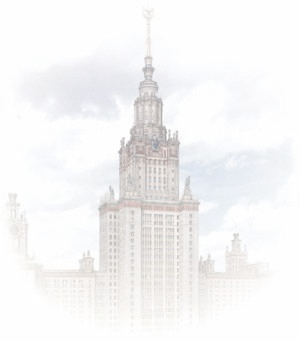
\includegraphics{img/msu}
% \end{center}
 }
 \renewcommand{\ESKDtheTitleFieldIV}{
 \parbox[r][5cm]{5cm}{}
 
 \ESKDtheTitle}
 \renewcommand{\ESKDtheTitleFieldVIII}{
 \parbox[r][2.5cm]{5cm}{}
 
 \begin{flushright}
   \parbox[r]{5cm}{
     \ESKDtheAuthor
 
     Группа 422
 
     кафедра АСВК
 
     \textbf{Научный руководитель}
 
     к.ф.-м.н.,с.н.с. Гамаюнов Д.Ю.
   }
 \end{flushright}
 
 }
 \renewcommand{\ESKDtheTitleFieldX}{Москва \ESKDtheYear}

%  \begin{titlepage}
%   \begin{center}
%   \textsc{\LARGE{\textbf{Московский государственный университет}} \\[.5cm]
%  \large{\textbf{Факультет вычислительной математики и кибернетики} \\
%  \large{\textbf{Кафедра автоматизации систем вычислительных комплексов}} }} \\[4cm]
% 
% \bigskip
% 
% \bigskip
% 
% \bigskip
% 
% 
%   {\Large{\textbf{Инструментальное средство автоматизации построения моделей
%  нормального поведения приложений}}} \\[3cm]
%   \begin{flushright}
%   \textbf{Горнак Татьяны} \\
%   Группа 521\\
%   \textbf{Научный руководитель:}\\
%  к.ф.-м.н., м.н.с. Гамаюнов Д.Ю.
%  \end{flushright}
%  \vfill
%  Москва, 2010
%  \end{center}
% \end{titlepage}

\usepackage{courier}
\lstset{
    basicstyle=\footnotesize\ttfamily, % standardschrift
        %numbers=left,               % ort der zeilennummern
        numberstyle=\tiny,          % stil der zeilennummern
        %stepnumber=2,               % abstand zwischen den zeilennummern
        numbersep=5pt,              % abstand der nummern zum text
        tabsize=2,                  % groesse von tabs
        extendedchars=true,         %
        breaklines=true,            % zeilen werden umgebrochen
        keywordstyle=\color{red},
        frame=b,         
        %        keywordstyle=[1]\textbf,    % stil der keywords
            %        keywordstyle=[2]\textbf,    %
            %        keywordstyle=[3]\textbf,    %
            %        keywordstyle=[4]\textbf,   \sqrt{\sqrt{}} %
            stringstyle=\color{white}\ttfamily, % farbe der string
            showspaces=false,           % leerzeichen anzeigen ?
            showtabs=false,             % tabs anzeigen ?
            xleftmargin=17pt,
        framexleftmargin=17pt,
        framexrightmargin=5pt,
        framexbottommargin=4pt,
        %backgroundcolor=\color{lightgray},
        showstringspaces=false      % leerzeichen in strings anzeigen ?        
}
\lstloadlanguages{% check dokumentation for further languages ...
    %[visual]basic
        %pascal
        c
        %c++
        %xml
        %HTML
        %Java
}
%\DeclareCaptionFont{blue}{\color{blue}} 

%\captionsetup[lstlisting]{singlelinecheck=false, labelfont={blue}, textfont={blue}}
\usepackage{caption}
\DeclareCaptionFont{white}{\color{white}}
\DeclareCaptionFormat{listing}{\colorbox[cmyk]{0.43, 0.35, 0.35,0.01}{\parbox{\textwidth}{\hspace{15pt}#1#2#3}}}
\captionsetup[lstlisting]{format=listing,labelfont=white,textfont=white, singlelinecheck=false, margin=0pt, font={bf,footnotesize}}
\usetikzlibrary{calc}

\begin{document}
\maketitle


\large{\textbf{АННОТАЦИЯ}}

В работе рассматривается возможность расширения функциональности
механизма контроля поведения программ, используемого в SELinux
(SEAndroid на платформе Android), при помощи повышения гранулярности
контроля поведения приложений в указанной системе за счет отслеживания
внутреннего состояния программы из ядра. Предлагается реализация данной
возможности на ОС Android.

\newpage

\tableofcontents
\newpage

%\begin{titlepage}
	\begin{center}
	\textsc{\large{Московский государственный yниверситет им.~М.В.~Ломоносова}
	\normalsize{Факультет вычислительной математики и кибернетики\\
	Кафедра автоматизации систем вычислительных комплексов}}

	{\Large {Контроль поведения приложений в SEAndroid}} \\[3cm]
	\begin{flushright}
                курсовая работа студента 422 группы
		Бушмакина П.С.\\
		
		Научный руководитель:\\ 
		Гамаюнов Д.Ю.
	\end{flushright}
	\vfill
	
	Москва, 2013 г.
	\end{center}

\end{titlepage}


 \tikzstyle{pil}=[ ->,
	thick,
	shorten <=2pt,
	shorten >=2pt]

\tikzstyle{de} = [diamond, drawshade, top color=white,
    bottom color=blue!50!black!20, draw=blue!40!black!60, very
    thick, text centered, rounded corners, text width=6em, text badly centered, node distance=3cm, inner sep=0pt]

 \tikzstyle{decision} = [diamond, drawshade,  top color=white,
    bottom color=blue!50!black!20, draw=blue!40!black!60, very
    thick, text width=4.5em, text badly centered, node distance=3cm, inner sep=0pt]

 \tikzstyle{block} = [rectangle, draw,  text width=5em, text centered, minimum height=4em, top color=white,  bottom color=blue!50!black!20, draw=blue!40!black!60, very thick, rounded corners]

\tikzstyle{line} = [draw, -latex']
\tikzstyle{cloud} = [draw, ellipse,fill=red!20, node distance=3cm,
    minimum height=2em]
   
\tikzset{blue dotted/.style={draw=blue!50!white, line width=1pt,
                               dash pattern=on 1pt off 4pt on 6pt off 4pt,
                                inner sep=4mm, rectangle, rounded corners}}
\tikzstyle{blockwhite} = [rectangle, draw,  text width=5em, text centered, minimum height=4em, draw=white, fill=white]
\tikzstyle{bl} = [block, shade, top color=white,
    bottom color=blue!50!black!20, draw=blue!40!black!60, very
    thick, text width=10em, text centered, rounded corners, minimum height=4em]

\tikzstyle{step} = [ elipse, text width=5em, text centered, minimum height=4em,top color=white,
    bottom color=blue!50!black!20, draw=blue!40!black!60, very thick]

\bigskip 
\section{Введение.}

Механизмы разграничения доступа на уровне операционной
системы исторически являются одним из основных способов
обеспечения информационной безопасности, не менее
важным, чем криптография. Именно ядро операционной системы
и встроенные в него механизмы обеспечивают выполнение
кода процессов на аппаратуре и контролируют доступ
процессов к ресурсам.

Традиционной для UNIX-подобных систем является дискреционная
модель разграничения доступа. 

В 1985 году был введен стандарт «Критерии 
оценки доверенных компьютерных систем» более известный 
под названием «Оранжевая книга». Данный стандарт получил 
международное признание и оказал сильное влияние на 
последующие разработки в области информационной безопасности. 
Появилось семейство так называемых "trusted" операционных 
систем — TrustedBSD, Trusted Solaris, Trusted UNICOS 8.0, 
HP-UX 10.26, PitBull for AIX 5L, XTS-400. На сегодняшний 
день результатами разработки 
более современных и продвинутых систем безопасности, 
работающих поверх стандартных, стали такие продукты, как 
SELinux (NSA, Red Hat)~\cite{SEOF}, AppArmor (Immulinux, Novell) 
~\cite{AppArmor},
GRSecurity\cite{pax}, Seatbelt(Apple).

В случае SELinux контроль контроль основан на
описании набора типов объектов и субъектов, где для
каждого типа субъектов в явном виде описаны все разрешённые
операции над типами объектов. Во время запуска приложения
ему принудительно присваивается один из типов субъектов.

Для каждого из типов субъектов работает принцип наименьших
привилегий, который гласит, что любой субъект в системе
должен иметь возможность получить доступ к тем и только к
тем объектам, которые ему необходимы для нормального
функционирования. Подобное решение является оправданным,
так как на практике большинству приложений требуется лишь
небольшое подмножество привилегий, которыми обладает
пользователь. В результате компрометация приложения
злоумышленником не несет в себе угрозы целостности
и конфиденциальности данных пользователя, к которым не
имеет доступа скомпрометированное приложение. Это является
существенным улучшением традиционной традиционной
модели безопасности, существующей в UNIX-подобных системах.

Реализованный в AppArmor и SELinux способ контроля предполагает
предоставление приложению одних и тех же привилегий с момента
запуска и до его завершения. При этом в большинстве приложений
на разных стадиях выполнения минимальный набор необходимых
привилегий может различаться. В качестве примера можно привести
сетевые приложения, где, как правило, доступ к файлам конфигурации
требуется только непосредственно после запуска приложения,
а в процессе авторизации пользователя нужен лишь доступ к сети и
объектам, необходимым для авторизации. После успешной авторизации
пользователя набор прав приложения, как правило, должен существенно
расшириться.

В результате, ограничения накладываемые на поведение приложений,
могут являться избыточными, но их невозможно сократить без потери
нормального функционирования приложения. Таким образом, возникает
идея динамически изменять набор привилегий приложения в зависимости
от состояния его исполнения.
 
\newpage
\section{Постановка задачи}
\begin{comment}
\subsection{Расшифровка темы}
Завершение работ 3 курса и работ Торощина,
Сапожникова, Горнак по отслеживанию поведения приложений со стороны ядра
ОС с помощью расстановки отладочных меток, сопоставления наблюдаемых
трасс с предварительно построенной моделью поведения и переключению
текущего профиля SELinux при изменениях состояния приложения.
Демонстрация reference implementation на примере популярного приложения
с искуственно внесённой уязвимостью. Публикация проекта.
\end{comment}

Разработать и реализовать набор инструментов для
разметки приложений (исходного кода и соответствующих бинарных программ)
контрольными точками (software breakpoints), разработать и реализовать
подсистему ядра Линукс, способную отслеживать поведение приложения в
виде последовательности системных вызовов и проходов через контрольные
точки, сопоставлять его с предварительно построенной автоматной моделью
и переключать активный профиль SELinux приложения при изменении его
состояния.

\begin{comment}
\subsection{Детализация постановки}
Для решения поставленной задачи необходимо решить следующие подзадачи:
\begin{itemize}
\item Разработать и реализовать набор инструментов для установки
контрольных точек в программе, а также динамической установки таких
точек в работающей программе.
\item Выбрать пример сетевого приложения, в котором: а) есть удалённо
эксплуатируемая уязвимость, б) данная уязвимость позволяет нарушить
конфиденциальность, целостность или доступность системы в случае
компрометации даже при наличии политики SELinux (контрпример к SELinux).
Показать, как можно расставить контрольные точки в данном приложении,
чтобы ущерб от атаки был минимальным.
\item Разработать и реализовать механизм наблюдения за поведением со
стороны ядра, отладить на выбранном примере сетевого приложения.
\item Опубликовать проект в публичном репозитории и в тематических списках
рассылки.
\end{itemize}

\subsection{Ожидаемые результаты}
\begin{itemize}
\item Набор утилит для расстановки контрольных точек, с использованием
результатов работы Татьяны Горнак прошлого года.
\item Набор модулей ядра, реализующий контроль поведения и переключение
контекстов SELinux, желательно с минимальными модификациями кода ядра.
\item Публичный репозиторий со всем, что необходимо стороннему пользователю
для того, чтобы воспользоваться результатами работы.
\end{itemize}

\end{comment}
\section{Формальная постановка задачи}

\subsection{Основные понятия и определения}
Обозначим: 

$\mathcal{S} - \text{множество системных вызовов,}$

$\mathcal{R} - \text{множество ресурсов системы.}$

Каждому ресурсу  соответствует конечный набор операций доступа, 
например, по открытию, чтению, записи и т.д. Такими операциями
доступа являются системные вызовы.

\textbf{Правило  SELinux для программы ($\mathcal{D}$)} -- отображение пары: системный вызов, ресурс на реакцию системы на правило:

$$\mathcal{D}: s \times r \to \{accept, decline\}, s \in \mathcal{S}, r \in \mathcal{R} \text{, где} $$\\
$accept$ -- разрешить выполнить системный вызов $s$ над ресурсом $r$,\\
$decline$ -- запретить выполнение.

\textbf{Модель программы} -- граф потока управления программы,
преобразованный таким образом, что его вершины представляют собой
различные участки программы, которым соответствует различное множество
наименьших привилегий, а переходы соответствуют переходам между данными
участками.

\textbf{Контрольная точка} -- Адрес в сегменте кода виртуального адресного
пространства процесса, попадание исполнения на который символизирует о
переходе модели программы в новое состояние.

\subsection{Постановка задачи}

Дано -- модель программы. Требуется:

\begin{itemize}
\item Разработать и реализовать набор инструментов для установки
контрольных точек в программе, а также динамической установки таких
точек в работающей программе.
\begin{comment}
\item Выбрать пример сетевого приложения, в котором: а) есть удалённо
эксплуатируемая уязвимость, б) данная уязвимость позволяет нарушить
конфиденциальность, целостность или доступность системы в случае
компрометации даже при наличии политики SELinux (контрпример к SELinux).
Показать, как можно расставить контрольные точки в данном приложении,
чтобы ущерб от атаки был минимальным.
\end{comment}
\item Разработать и реализовать механизм наблюдения за поведением со
стороны ядра, отладить на выбранном примере сетевого приложения.
\item Продемонстрировать работу реализованной системы на сетевом приложении,
    в котором существует:
    \begin{itemize}
    \item удалённо эксплуатируема уязвимость
    \item данная уязвимость позволяет нарушить конфиденциальность, целостность
        или доступность системы в случае компрометации даже при наличии политики
        SELinux
    \end{itemize}
\end{itemize}

\section{Обзор существующих систем безопасности 
    уровня ядра ОС Linux и ОС Trusted BSD}

\bigskip
Сравним системы безопасности уровня ядра ОС Linux
(SELinux, AppArmor, GRSecurity) и Trusted BSD. 
Для сравнительного анализа были выбраны следующие 
критерии:

\bigskip
{\bfseries Реализованные модели безопасности.} 

    Существуют различные модели безопасности такие, 
    как Дискреционная(DAC), Мандатная(MAC), Принудительное 
    присвоение типов на основании определенной 
    политики(TE), Списки контроля доступа(ACL). 
    Данный критерий отражает реализованные 
    в рассматриваемой системе модели безопасности.  

\bigskip
{\bfseries Наличие возможности изменять матрицу доступа 
	во время исполнения.}
	
	Во многих из упомянутых выше моделях безопасности 
	котроль событий в системе осуществляется на основании 
	матрицы доступа. Матрица доступа является отображением 
	декартова произведения множеств объектов и субъектов 
	системы на множество, элементами которого являются 
	наборы прав.
	Критерий отражает, есть ли возможность изменять
	матрицу доступа во время исполнения. 

\bigskip 
{\bfseries Возможность динамической смены контекстов
	приложения.}
	
	Для учета внутреннего состояния приложения в 
	процессе контроля за его поведением может быть
	использована динамическая смена конекста безопасности 
	 приложения. 
	Критерий описывает, существует ли в рассматриваемой 
	системе возможность менять права приложения в процессе
	исполнения. 

\bigskip
{\bfseries Классы вредоносных действий, предотвращаемых 
	системой безопасности.}
	
	Разные системы безопасности предотвращают различные 
	классы вредоносных действий. Некоторые системы 
	идут по пути предотвращения заранее известных 
	действий злоумышленника, другие позволяют минимизировать 
	нанесенный ущерб от успешной атаки. Из-за этого на практике 
	часто приходится комбинировать различные системы безопасности.    

\bigskip
\subsection{SELinux} 
SELinux является системой безопасности 
уровня ядра Linux, основанной на 
подсистеме LSM. LSM позволяет 
создавать модули безопасности. Данные модули 
должны реализовывать 
определенную логику принятия решений о 
разрешении или запрещении различных 
взаимодействий между объектами и субъектами 
системы. 

Под объектами системы здесь 
понимаются файлы, объекты межпрограммного 
взаимодействия, объекты сетевого взаимодействия 
и прочие. Субъекты представляют собой 
пользовательские процессы, демоны, ядро и.т.д..

SElinux обеспечивает возможность 
комплексной защиты системы, ограничивая поведение 
приложений и пользователей в рамках политик 
безопасности. В первую очередь, SELinux 
направлена на борьбу с успешными атаками, 
в частности, с атаками нулевого дня, когда 
уязвимость уже известна злоумышленнику, 
но лекарства еще не было выпущено. В таких 
случаях уязвимость локализируется на уровне 
политики. Компания Tresys ведет подсчет 
конкретных случаев угроз безопасности, которые, 
в частности, могли быть предотвращены SELinux. 
В их числе: переполнение буфера в Samba (may 
2007), Apache DoS (jun 2007), Mambo exploit (jul 
2007), hplip Security flaw (oct 2007). 

Конфигурация политик является 
сложной задачей из-за необходимости
описывать профили для каждого приложения 
вручную на на специальном языке описания
политик. Добавление новых профилей может повлечь 
за собой необходимость в модификации уже имеющихся 
профилей, что может привести к появлению 
ошибок и росту накладных расходов на 
администрирование системы.  

Схема работы SELinux заключается в следующем.
Имеется политика, описывающая типы обеъектов
и субъектов в системе и матрицу доступа,
содержащую для каждого из субъектов его права
на операции с любым из типов объектов. Когда
любой из процессов производит системный вызов
для доступа к какому-либо объекту, подсистема
ядра SELinux вычисляет, имеет ли тип данного процесса
права на доступ к типу запрашиваемого объекта.
Если таких прав нет, запрашивающему процессу
будет отказано в доступе к объекту. В противном
случаe, доступ к объекту будет предоставлен.
Схематично работа SELinux изображена на рисунке
\ref{fig:selinux}.

\begin{figure}
\centering
\subfloat{\label{fig:selinux}{\begin{tikzpicture}[->,<->,>=latex,grow=right]

\tikzstyle{state} = [draw,rounded corners, fill=white, rectangle, minimum height=3em, minimum width=5em, node distance=7em, font={\sffamily\small}]
\tikzstyle{stateEdgePortion} = [black,thick];
\tikzstyle{stateEdge} = [stateEdgePortion,->, minimum width=10em,node distance=8em];
\tikzstyle{shitEdge} = [stateEdgePortion,<->, minimum width=10em,node distance=8em];
\tikzstyle{edgeLabel} = [pos=0.5, text centered, font={\sffamily\small}];

\node[state, name=server] {SELinux};
\node[state, name=subject, left of=server,xshift=-6em] {Процесс};
\node[state, name=policy, below of=server, yshift=2em] {Политика};
\node[state, name=acl, right of=server] {Есть ли права?};
\node[state, name=notGranted, below of=acl,xshift=1em, yshift=2em] {Отказать в доступе};
\node[state, name=granted, right of=acl, xshift=3em] {Разрешить доступ};

\draw[->](subject) edge[stateEdge] node[edgeLabel,yshift=0.5em] {\emph{Системный вызов}} (server);
\draw[<->](server) edge[shitEdge] node[edgeLabel, xshift=-3.3em,yshift=0em] {\emph{Проверка прав}} (policy);
\draw[->](server) edge[stateEdge] node[edgeLabel,yshift=0.5em] {} (acl);
\draw[->](acl) edge[stateEdge] node[edgeLabel,xshift=1em,yshift=0.3em] {\emph{Нет}} (notGranted);
\draw[->](acl) edge[stateEdge] node[edgeLabel,yshift=0.5em] {\emph{Есть}} (granted);
\end{tikzpicture}
}}
\caption{Схема работы подсистемы безопасности ядра SELinux}
\end{figure}

\subsubsection{Пример политики SELinux}

В качестве примера политики SELinux можно привести
фрагмент политики приложения OpenSSH.

\lstinputlisting[label=samplecode13,caption=Пример конфигурации модуля SELinux]{sourceCode/sepol.txt}
В данном фрагменте описывается тип процесса ssh\_t и
набор привилегий, предоставляемых данному типу:
\begin{itemize}
\item Set capability
\item Отлаживать процессы типа ssh\_t, исполнять свои сегменты
        кучи и стека
\item Использовать очереди сообщений
\item Отправлять и посылать сообщения
\item Использовать сокеты
\end{itemize}

\subsubsection {Реализованные модели безопасности.} 

Принудительное присвоение типов (TE). 

Основной идеей принудительного присвоения
типов является явная разметка всех объектов 
в системе специальными структурами данных 
(метками безопасности), хранящими в себе информацию
об атрибутах объекта, используемую при принятии 
решений внутри логики политики. 
Для процессов и объектов используется 
один и тот же тип атрибутов. Поэтому достаточно 
одной матрицы для описания взаимодействий между 
разными типами, при этом объекты одного типа могут 
рассматриваться по-разному, если их их ассоциированные 
классы безопасности различны. Пользователи не 
привязаны к типам безопасности напрямую, вместо 
этого используется RBAC.

\bigskip
Ролевой контроль доступа (RBAC) 

Данный метод используется для определения 
множества ролей, которые могут 
быть назначены пользователям. SELinux расширяет 
модель RBAC до жесткой привязки пользовательских 
ролей к определенным доменам безопасности, роли 
могут быть организованы в виде иерархии приоритетов. 
Такая привязка ролей к доменам позволяет принимать 
большинство решений на основе конфигурации TE. 
Контекст безопасности, кроме всего прочего, включает 
в себя атрибут роли.

\bigskip
Многоуровневая система безопасности (MLS) 

SELinux предоставляет MLS для случаев, когда есть 
необходимость в традиционной многоуровневой системе 
безопасности. У объектов и субъектов могут быть 
различные уровни и категории. 
Как правило, используется лишь один уровень. 


\subsubsection{Наличие возможности изменять матрицу доступа 
	во время исполнения} 

SELinux Предоставляет возможность перезагружать 
	политику во время работы системы. 

\subsubsection{Возможность динамической смены контекстов 
приложения} 
 
SELinux предоставляет разработчикам приложений 
инструментарий, позволяющий создавать более 
безопасные приложения. Этого можно достичь 
путем изменения текущих привилегий приложения 
во время его исполнения. 
Последнее реализуется путем изменения домена приложения. 
Приложение должно запросить у ядра ОС смену своего 
текущего домена на указанный. При этом возможность
такой смены доменов должна быть явно описана в 
политике безопасности. Далее данный метод будет
рассмотрен более подробно.  

\subsubsection{Классы вредоносных действий, предотвращаемых 
	системой безопасности} 

В отношении системы безопасности SELinux было бы неправильно 
говорить о предотвращении угроз. Кроме этого, система не 
оперирует классами угроз. Основной идеей SELinux является 
минимизация ущерба от успешных атак на приложение. Для 
этого накладываются жесткие рамки на поведение приложений. 


\begin{comment}
\subsubsection{Принципы работы}

Главными элементами системы безопасности 
являются субъект, объект и действия. В классы 
объектов входят классы файлов (blk\_file, chr\_
file, dir, fd,...\ ) ,  классы межпрограммного 
взаимодействия (ipc,msg,msgq,sem,shm), классы 
сетевого взаимодействия (key\_socket,netif,node,
packet\_socket,tcp\_socket), классы объектов 
(passwd), системные классы (capability, process,
Secutity, System). Под субъектами понимаются 
процессы, демоны, ядро и.т.д.. Действия, которые субъекты 
SELinux могут производить над объектами 
различны для различных классов объектов. 
Для классов файлов это, например, 
будут создание, исполнение, ссылки, чтение, запись, 
удаление. 

SELinux ассоциирует атрибуты безопасности 
с субъектами и объектами и основывает свои решения 
на этих атрибутах. Атрибутами являются: идентификатор 
пользователя, роль и тип. Идентификатор пользователя 
— пользовательская учетная запись, ассоциированная с 
субъектом или объектом. У каждого пользователя может 
быть несколько ролей, но в какой-то конкретный момент
времени ему может быть предписана только одна из них. 
Пользователь может менять роли командой newrole. Типы 
(для процессов~--- Домены) делят субъекты и объекты на родственные 
группы. Это~--— главный атрибут безопасности, используемый 
SELinux для принятия решений. 

Типы позволяют помещать 
процессы в "песочницы" и предотвращать повышение 
привилегий. К примеру, роль суперпользователя - 
sysadm\_r, его тип — sysadm\_t. Политика безопасности 
SELinux загружается системой из бинарного файла политики,
который, как правило, находится в /etc/selinux. 
Бинарная политика собирается при помощи make, исходные 
коды, как правило, находятся в /etc/selinux/\$(POLNAME)/src/policy.

Инструменты работы с SELinux могут быть разделены на 
три категории: специальные утилиты для настройки и 
использования SELinux, модифицированные версии стандартных 
команд и программ Linux, некоторые добавочные инструменты,
к примеру, для настройки и анализа политик. Среди основных 
команд можно выделить следующие: chcon – помечает файл или 
группу файлов указанным контекстом безопасности, checkpolicy
– позволяет выполнять множество действий, связанных с 
политиками, в том числе, компиляцию политики и ее загрузку 
в ядро; getenforce — позволяет узнать в каком режиме 
работает SELinux, newrole – позволяет пользователю 
перемещаться между ролями; run\_init — позволяет 
запускать, останавливать или контролировать сервис; 
setenforce позволяет менять режим работы системы; 
setfiles присваивает метки указанной директории и ее 
поддиректориям. Некоторые из измененных программ: cron, 
login, logrotate, pam, ssh. Некоторые инструменты: Apol 
– инструмент для анализа файла policy.conf; SeAudit – 
инструмент для анализа логов, имеющий графический интерфейс; 
SeCmds; SePCuT — инструмент для просмотра и редактирования 
файлов политик; SeUser — модификация пользовательских 
учетных записей. 
\end{comment}

\subsubsection{Вывод}


\section{Обзор существующих систем контроля доступа в ОС Android и Linux}

\bigskip
Сравним системы контроля доступа для приложений в ОС Android.
Родственная природа Android и GNU/Linux позволяет также рассуждать о
более широком круге систем контроля доступа, а именно представленных в
Linux, но отсутствующих в Android. Для рассмотрения были выбраны Unix
DAC, SELinux, TOMOYO и XManDroid. Для сравнительного анализа были
выбраны следующие критерии:

\bigskip
{\bfseries Реализованные модели безопасности.} 

    Существуют различные модели безопасности такие, как
    Дискреционная(DAC), Мандатная(MAC), Принудительное присвоение типов
    на основании определенной политики(TE), Списки контроля
    доступа(ACL).  Данные модели были определены в \cite{orangebook} и
    являются де-факто стандартами при описании систем безопасности.

\bigskip
{\bfseries Наличие возможности изменять матрицу доступа 
	во время исполнения.}
	
    Во многих из упомянутых выше моделях безопасности контроль событий в
    системе осуществляется на основании матрицы доступа. Матрица доступа
    это отображение декартова произведения множеств объектов и субъектов
    системы на множество, элементами которого являются наборы прав.
    Критерий отражает, есть ли возможность изменять матрицу доступа во
    время исполнения. 

\bigskip
{\bfseries Классы вредоносных действий, предотвращаемых 
	системой безопасности.}
	
    Разные системы безопасности предотвращают различные классы
    вредоносных действий. Некоторые системы идут по пути предотвращения
    заранее известных действий злоумышленника, другие позволяют
    минимизировать нанесенный ущерб от успешной атаки. Из-за этого на
    практике часто приходится комбинировать различные системы
    безопасности.    

\bigskip
\subsection{Unix DAC} 
Контроль доступа на основе Дискреционной модели безопасности является
классическим способом разграничения привилегий в UNIX-подобных системах.
В основе подхода лежит принадлежность объектов в системе некоторым
субъектам, называемым владельцами объекта. Именно владелец объекта 
определяет права на доступ к своему объекту другим пользователям в
системе. Объект также принадлежит определённой группе пользователей, но
никто из них не имеет привилегий владельца.

В UNIX существует 3 группы пользователей для которых владелец
может определить права доступа: для владельца, для владеющей группы
и для всех остальных пользователей. Права на доступ к объекту делятся на
3 вида: права на чтение, запись и исполнение. Такое распределение можно
объяснить тем, что каждый объект в UNIX имеет интерфейс, подобный тому,
что есть у файлов: из файла можно прочитать содержимое, можно записать,
а можно исполнить записанную в нём программу. Помимо определения прав
доступа, владелец может передать свои права владения другому
пользователю или определить новую владеющую группу. Для доступа
приложения к специальным операциям, пользователю могут быть
гарантированы права из UNIX capabilities. Предоставляются возможности
для смены своего UID (пользователь может стать другим пользователем),
права на обход проверки привилегий чтения, записи и исполнения,
возможности по созданию файлов устройств, возможность посылать пакеты в
обход стека tcp/ip (т.е. в обход стандартных системных вызовов,
генерирующих заголовки tcp/ip), выполнение chroot, монтирование файловых
систем, отладка процессов и др. 

Доступ к объекту приложениям предоставляется следующим образом: каждое
исполняемое в системе приложение имеет эффективный идентификатор
пользователя, который определяет, от имени какого пользователя
исполняется данное приложение; когда приложение запрашивает у системы
некоторый ресурс(например, посредством системного вызова), последняя
определяет связанный с ресурсом объект, а также под какую группу прав
подпадает запрашиваемый доступ, затем в матрице доступа по паре
пользователь-объект определяется запись, где содержатся допустимые
права, если запрошенный доступ соответствует разрешённому, то система
предоставляет приложению доступ к ресурсу, иначе выдаёт сообщение об
ошибке.

В системе также имеется специальный пользователь, называемый root,
имеет права супер-пользователя, т.е. может выполнять любые действия над
объектами вне зависимости от их принадлежности. Также пользователю root
делегированы особые права, невозможные для получения другими
пользователями. Сюда входит например возможность, создавать слушающее
соединение на сетевых портах из диапазона 1-1024, который считается
зарезервированным за основными протоколами. Так как некоторым
пользовательским приложениям порой бывают нужны такие права, UNIX DAC
даёт право супер-пользователю выставлять так называемый SetUID-бит для
объекта системы: приложение, запускаемое из такого объекта владеет
правами супер-пользователя, при этом владельцем объекта остаётся обычный
пользователь, а значит он может запускать данное приложение.

\subsubsection {Реализованные модели безопасности.} 

Как следует из названия UNIX DAC реализует только дискреционную модель
безопасности. В рамках данной модели пользователи сами устанавливают
политики доступа к своим объектам.

\subsubsection{Наличие возможности изменять матрицу доступа 
	во время исполнения} 

Пользователи могут в изменять права на доступ к объекту и передавать
право владения другим пользователям.

\subsubsection{Классы вредоносных действий, предотвращаемых 
	системой безопасности} 

Система предназначена для минимизации ущерба в случае успешных атак на
приложение. Однако в части сохранения секретности данных отдельных
пользователей могут наблюдаться проблемы. Основной принцип дискреционной
модели направлен на баланс между безопасностью и простотой
администрирования, ведь ответственность за объекты пользователей
оставлена на их совести. Если пользователь неправильно определит права
на доступ к объекту из вне, то возможны успешные атаки на
конфиденциальность. Модель также плоха в окружениях, где требуется
жёсткий контроль администратора, например в системах, где уровень
секретности данных, с которыми работают пользователи высок. В случае
атак по сговору пользователь системы может нарочно ослабить защищённость
секретной информации. Общая простота модели с файловыми объектами и 3
группами прав также несёт в себе опасность, так как нет возможности
более тонко ограничить права приложений. Такая простота приводит к тому,
что системным сервисам, решающим важные задачи функционирования системы
(сетевые серверы, мониторинг и логгирование, ipc, БД) приходится выдавать
права root для их нормального функционирования. Успешные атаки на
root-приложения приводят к существенным проблемам при эксплуатации их
привилегий. 

\bigskip
\subsection{SELinux} 

SELinux система контроля доступа, работающая на уровне ядра операционной
системы. Допустимые права приложений определяются на основе политик
безопасности. В задачу системы входит ограничение прав работающих
приложений для минимизации ущерба от атак. SELinux даёт централизованный
контроль над каждым исполняемым приложением и работает по принципу "что
не разрешено, то запрещено". Одним из главных преимуществ использования
SELinux является широкая описательная возможность политик безопасности,
которая позволяет задавать доступ к ресурсам по принципу минимальных
привилегий. SELinux базируется на Linux Security Modules (LSM, более
подробно см. в \cite{LSM}), эта система отвечает за отслеживание всех
точек доступа к ресурсам операционной системы через так называемые
"хуки" в системных вызовах.  При попадании исполнения системного вызова
на такой хук, LSM выполняет проверку прав доступа приложения на
возможность выполнения этого системного вызова сначала через
классическую систему Дискреционного Контроля Доступа (DAC), а затем
обращается к SELinux.

Модель SELinux оперирует следующими основными понятиями: 
\begin{description}
    \item{Тип} \hfill \\
        Определяет группу сущностей(процессов, файлов, сокетов и т.д.).
        Для процессов тип имеет специальное название — \emph{Домен}. На
        основе политики безопасности в SELinux определяется какие
        операции представители одного типа могут производить над
        представителям другого.  
    \item{Объект}  \hfill \\
        Сущность, через которую информация проходит к субъекту. Это
        могут быть каталоги, файлы, поля, экраны, клавиатуры, память,
        магнитные накопители, принтеры или любые другие устройства
        хранения/перемещения данных. В сущности это контейнер данных или
        ресурс системы, доступ к объекту фактически означает доступ к
        данным.  
    \item{Cубъект}  \hfill \\
        Любая активная сущность, вызывающая перемещение информации между
        объектами, т.е.  пользователь, пользовательский обработчик,
        системный процесс и т.д.  
    \item{Атрибут}  \hfill \\
        Абстракция операции или группы операций, которые субъект может
        выполнить над объектом, например, чтение процессом файла.  
    \item{Политика безопасности}  \hfill \\
        Набор правил определяющих возможности доступа субъектов к
        объектам. Правила представляются в виде тройки \{тип субъекта, тип
        объекта, атрибут\}. С помощью политик SELinux в системе можно
        реализовывать доступ на основе подходов разных формальных
        моделей безопасности: Role-Based Access Control (RBAC), Type
        Enforcement (TE), Multi-Level Security (MLS). TE является
        наиболее популярной в последнее время.   
    \item{Контекст}  \hfill \\
        Элемент правила политики безопасности, определяющий тип
        сущности. В случае TE это понятие эквивалентно типу.
\end{description}

Общий алгоритм принятия решений о предоставлении
доступа(проиллюстрирован на рисунке \ref{fig:selarch}): 
\begin{itemize}
\item Процесс пытается выполнить операцию над объектом 
\item Сервер принятия решений получает уведомление от LSM о попытке
    провести операцию, получает контексты субъекта и объекта, а также
    атрибут операции от LSM и передаёт эту информацию серверу политики в
    виде запроса 
\item Сервер политики сначала проверяет в кэше наличие решения для
    такого запроса: разрешить или запретить операцию. Если решение
    найдено оно возвращается серверу принятия решения. Иначе ищется
    соответствующее правило в политике безопасности и на основе его
    принимается решение, помещается в кэш и опять же возвращается
    серверу принятия решений. Если правила не найдено то принимается
    решение запретить 
\item Сервер принятия решений на основе информации от сервера политики
    либо запрещает исполнение операции приложением (в этом случае,
    например, системный вызов аварийно завершается с кодом ошибки), либо
    позволяет продолжение выполнения операции 
\end{itemize}

\subsubsection{Политика SELinux} 

В качестве примера политики SELinux можно привести
фрагмент политики приложения OpenSSH.

\lstinputlisting[label=samplecode13,caption=Пример конфигурации модуля SELinux]{sourceCode/sepol.txt}
В данном фрагменте описывается тип процесса ssh\_t и
набор привилегий, предоставляемых данному типу:
\begin{itemize}
\item Set capability
\item Отлаживать процессы типа ssh\_t, исполнять свои сегменты
        кучи и стека
\item Использовать очереди сообщений
\item Отправлять и посылать сообщения
\item Использовать сокеты
\end{itemize}

Политики позволяет описывать права на доступ к широкому ряду ресурсов
ОС. Гранулярность языка позволяет разрешать и запрещать выполнять
определённые системные вызовы по отношению к объектам системы. В
качестве объектов могут указываться файлы, устройства, сокеты, сетевые
порты, сетевые интерфейсы, ipc, файловые системы.  Правила политики
SELinux определяют неизменный набор привилегий для процесса с
соответствующим типом. Для изменения набора привилегий процессу
необходимо сменить тип, т.е. контекст. SELinux предоставляет для этого
несколько возможностей. Первая может быть определена в политике через
ключевое слово \emph{domain transition}. Такое правило определяет для
процесса возможность исполнять приложение другого типа (совершать
системный вызов execve). После того как новое приложение начнёт
исполнение, тип процесса будет изменён. Вторая возможность
предоставляется только для типов, у которых в политике задан атрибут
\emph{setattr}. Процессы такого типа могут совершать изменение своего
типа на любой другой, определённый в политике, с помощью библиотеки
libselinux.  Как видно, в политиках SELinux нет возможности описать
динамическое изменение привилегий процесса для произвольного типа.

\subsubsection {Реализованные модели безопасности.} 
SELinux реализует Мандатную модель безопасности, при это доступны к
применению различные её вариации:

Принудительное присвоение типов (TE). 

При таком подходе каждый объект и субъект в системе получает
принудительный идентификатор, который в дальнейшем используется для
принятия решений на основе политики. Данный идентификатор используется
для записи допустимых прав в политики безопасности. В TE субъектами
являются непосредственно приложения, а не пользователи которые их
запускают. В SELinux такой идентификатор называется типом для объектов и
доменом для приложений.  Типы всегда относятся к определённым классам,
которые определяют природу абстрактного ресурса, т.е. класс типа говорит
о том, какие с данным типом возможны операции. Также при описании
допустимого доступа между доменом и объектом может дополнительно
указываться класс, для чёткого описания природы взаимодействия, ведь
один и тот же объект может принадлежать разным классам, в которых
определены операции с одинаковыми по написанию, но различными по
действию операциями.

\bigskip
Ролевой контроль доступа (RBAC) 

Данный метод используется для определения множества ролей, которые могут
быть назначены пользователям. SELinux расширяет модель RBAC до жесткой
привязки пользовательских ролей к определенным доменам безопасности,
роли могут быть организованы в виде иерархии приоритетов.  

\bigskip
Многоуровневая система безопасности (MLS) 

SELinux предоставляет MLS для случаев, когда есть 
необходимость в традиционной многоуровневой системе 
безопасности. У объектов и субъектов могут быть 
различные уровни и категории. 
Как правило, используется лишь один уровень. 

\subsubsection{Наличие возможности изменять матрицу доступа 
	во время исполнения} 

Пользователи могут в изменять права на доступ к объекту и передавать
право владения другим пользователям.

\subsubsection{Классы вредоносных действий, предотвращаемых 
	системой безопасности} 

В отношении системы безопасности SELinux было бы неправильно 
говорить о предотвращении угроз. Кроме этого, система не 
оперирует классами угроз. Основной идеей SELinux является 
минимизация ущерба от успешных атак на приложение. Для 
этого накладываются жесткие рамки на поведение приложений. 

\bigskip
\subsection{TOMOYO Linux} 
TOMOYO Linux позволяет реализовать мандатный контроль доступа в системе
на основе анализа нормального поведения приложений и последующей
генерации политик безопасности. Реализованный в 2003 году, в качестве
Linux Security Module, TOMOYO Linux прошёл несколько ревизий, на данный
момент актуальной является версия 2.5. TOMOYO Linux предлагает
анализировать необходимые приложению ресурсы, а затем по собранной
информации сгенерировать политику безопасности, которая уже затем в
режиме MAC будет ограничивать его права в системе. В режиме обучения
TOMOYO Linux записывает информацию обо всех ресурсах которые приложение
запрашивает. Далее данный список анализируется составителем политик и
если все требования удовлетворены, генерируется политика.

Субъектами в TOMOYO являются процессы. Каждый процесс обладает доменом
исполнения, который определяет его права. Домен складывается из "истории
исполнения", т.е. из всех приложений, которые данный процесс исполнял,
включая историю потомков процесса. Приложение же идентифицируется по
пути в файловой системе его исполнительного файла (например, /sbin/ip).

Права же определяются в профилях. Чтобы предоставить права домену, нужно
добавить этот домен в профиль. Права могут задаваться над объектами,
описываемыми своим путём в файловой системе. Список возможных прав
включает в себя файловые операции (создание, удаление, чтение, запись,
исполнение, создание директорий, ссылок, фалов устройств, ipc),
монтирование файловых систем, chroot, операции с сетью. Для упрощения
работ с политиками используются исключения, применяемые вне зависимости
от того, какие профили управляют данным доменом.

\subsubsection {Реализованные модели безопасности.} 

В TOMOYO Linux реализована Мандатная модель безопасности.

\subsubsection{Наличие возможности изменять матрицу доступа 
	во время исполнения} 

История исполнения влияет доступные права, так что приложение может
иметь различные права. Есть возможность менять политику безопасности в
процессе исполнения.

\subsubsection{Классы вредоносных действий, предотвращаемых 
	системой безопасности} 

TOMOYO Linux прежде всего направлен на изучению требуемых приложениям
ресурсов, он также позволяет минимизировать ущерб в случае успешной
атаки, путём предоставления минимальных привилегий.


\bigskip
\subsection{XManDroid} 

XManDroid был предложен в \cite{xmandroid} и представляет собой систему
безопасности для Android, чьей целью является предотвращение атак по
сговору и атак типа confused deputy, при которых зловредное действие
может быть осуществлено силами нормального приложения, имеющего
необходимые права в системе, но обманным путём принуждённого к
совершению такового. Решение представляет собой комбинацию системного
монитора, выявляющего пути следования данных между приложениями,
политики безопасности, описывающие безопасные шаблоны поведения для
приложений, а также система MAC непосредственно гарантирующая права по
результатам решений системного монитора.  Системный монитор действует на
всех уровнях системы, отслеживая коммуникации через файлы и сокеты, ipc
и БД. При этом отслеживаются как прямые, так и связи через
представителей. Система динамически поддерживает информацию о связях
между приложениями, и каждый раз когда приложение выдаёт новый запрос на
взаимодействие с другим приложением, данный запрос оценивается на
соответствие политикам безопасности с учётом состояния системы, т.е.
предыдущих актов взаимодействия. Если системный монитор выявляет, что
данный запрос с учётом состояния системы не соответствует политике, то
доступ не предоставляется. В ином случае состояние системы обновляется,
отображая установленную связь. Мониторинг и обновление состояния
происходит как на уровне фреймворка приложений, так и на уровне ядра.

\subsubsection {Реализованные модели безопасности.} 

Используется Мандатная модель безопасности. При этом права на доступ
определяются не монолитно, а на основе действий приложений и сверки
с политиками безопасности, но сами политики применяются централизованно
и устанавливаются администратором.

\subsubsection{Наличие возможности изменять матрицу доступа 
	во время исполнения} 

Матрица доступа может меняться, в зависимости от состояния системы.

\subsubsection{Классы вредоносных действий, предотвращаемых 
	системой безопасности} 

XManDroid адресует атаки по сговору и confused deputy.

\begin{comment}

SELinux~--- система безопасности 
уровня ядра Linux, основанная на 
подсистеме LSM. LSM позволяет 
создавать модули безопасности. Данные модули 
должны реализовывать 
определенную логику принятия решений о 
разрешении или запрещении различных 
взаимодействий между объектами и субъектами 
системы. 

Под объектами системы здесь 
понимаются файлы, объекты межпрограммного 
взаимодействия, объекты сетевого взаимодействия 
и прочие. Субъекты представляют собой 
пользовательские процессы, демоны, ядро и.т.д..

SElinux обеспечивает возможность 
комплексной защиты системы, ограничивая поведение 
приложений и пользователей в рамках политик 
безопасности. В первую очередь, SELinux 
направлена на борьбу с успешными атаками, 
в частности, с атаками нулевого дня, когда 
уязвимость уже известна злоумышленнику, 
но лекарства еще не было выпущено. В таких 
случаях уязвимость локализируется на уровне 
политики. Компания Tresys ведет подсчет 
конкретных случаев угроз безопасности, которые, 
в частности, могли быть предотвращены SELinux. 
В их числе: переполнение буфера в Samba (may 
2007), Apache DoS (jun 2007), Mambo exploit (jul 
2007), hplip Security flaw (oct 2007). 

Конфигурация политик является 
сложной задачей из-за необходимости
описывать профили для каждого приложения 
вручную на на специальном языке описания
политик. Добавление новых профилей может повлечь 
за собой необходимость в модификации уже имеющихся 
профилей, что может привести к появлению 
ошибок и росту накладных расходов на 
администрирование системы.  

Схема работы SELinux заключается в следующем.
Имеется политика, описывающая типы объектов
и субъектов в системе и матрицу доступа,
содержащую для каждого из субъектов его права
на операции с любым из типов объектов. Когда
любой из процессов производит системный вызов
для доступа к какому-либо объекту, подсистема
ядра SELinux вычисляет, имеет ли тип данного процесса
права на доступ к типу запрашиваемого объекта.
Если таких прав нет, запрашивающему процессу
будет отказано в доступе к объекту. В противном
случае, доступ к объекту будет предоставлен.
Схематично работа SELinux изображена на рисунке
\ref{fig:selinux}.

\subsubsection {Реализованные модели безопасности.} 

Принудительное присвоение типов (TE). 

Основная идея принудительного присвоения
типов~--- явная разметка всех объектов 
в системе специальными структурами данных 
(метками безопасности), хранящими в себе информацию
об атрибутах объекта, используемую при принятии 
решений внутри логики политики. 
Для процессов и объектов используется 
один и тот же тип атрибутов. Поэтому достаточно 
одной матрицы для описания взаимодействий между 
разными типами, при этом объекты одного типа могут 
рассматриваться по-разному, если их их ассоциированные 
классы безопасности различны. Пользователи не 
привязаны к типам безопасности напрямую, вместо 
этого используется RBAC.

\bigskip
Ролевой контроль доступа (RBAC) 

Данный метод используется для определения 
множества ролей, которые могут 
быть назначены пользователям. SELinux расширяет 
модель RBAC до жесткой привязки пользовательских 
ролей к определенным доменам безопасности, роли 
могут быть организованы в виде иерархии приоритетов. 
Такая привязка ролей к доменам позволяет принимать 
большинство решений на основе конфигурации TE. 
Контекст безопасности, кроме всего прочего, включает 
в себя атрибут роли.

\bigskip
Многоуровневая система безопасности (MLS) 

SELinux предоставляет MLS для случаев, когда есть 
необходимость в традиционной многоуровневой системе 
безопасности. У объектов и субъектов могут быть 
различные уровни и категории. 
Как правило, используется лишь один уровень. 


\subsubsection{Наличие возможности изменять матрицу доступа 
	во время исполнения} 

SELinux Предоставляет возможность перезагружать 
	политику во время работы системы. 

\subsubsection{Возможность динамической смены контекстов
приложения} 
 
SELinux предоставляет разработчикам приложений 
инструментарий, позволяющий создавать более 
безопасные приложения. Этого можно достичь 
путем изменения текущих привилегий приложения 
во время его исполнения. 
Последнее реализуется путем изменения домена приложения. 
Приложение должно запросить у ядра ОС смену своего 
текущего домена на указанный. При этом возможность
такой смены доменов должна быть явно описана в 
политике безопасности. Далее данный метод будет
рассмотрен более подробно.  

\subsubsection{Классы вредоносных действий, предотвращаемых 
	системой безопасности} 

В отношении системы безопасности SELinux было бы неправильно 
говорить о предотвращении угроз. Кроме этого, система не 
оперирует классами угроз. Основной идеей SELinux является 
минимизация ущерба от успешных атак на приложение. Для 
этого накладываются жесткие рамки на поведение приложений. 

\section{Обзор SELinux и SEAndroid}

\newpage

\subsubsection{Принципы работы}

Главными элементами системы безопасности 
являются субъект, объект и действия. В классы 
объектов входят классы файлов (blk\_file, chr\_
file, dir, fd,...\ ) ,  классы межпрограммного 
взаимодействия (ipc,msg,msgq,sem,shm), классы 
сетевого взаимодействия (key\_socket,netif,node,
packet\_socket,tcp\_socket), классы объектов 
(passwd), системные классы (capability, process,
Secutity, System). Под субъектами понимаются 
процессы, демоны, ядро и.т.д.. Действия, которые субъекты 
SELinux могут производить над объектами 
различны для различных классов объектов. 
Для классов файлов это, например, 
будут создание, исполнение, ссылки, чтение, запись, 
удаление. 

SELinux ассоциирует атрибуты безопасности 
с субъектами и объектами и основывает свои решения 
на этих атрибутах. Атрибутами являются: идентификатор 
пользователя, роль и тип. Идентификатор пользователя 
— пользовательская учетная запись, ассоциированная с 
субъектом или объектом. У каждого пользователя может 
быть несколько ролей, но в какой-то конкретный момент
времени ему может быть предписана только одна из них. 
Пользователь может менять роли командой newrole. Типы 
(для процессов~--- Домены) делят субъекты и объекты на родственные 
группы. Это~--— главный атрибут безопасности, используемый 
SELinux для принятия решений. 

Типы позволяют помещать 
процессы в "песочницы" и предотвращать повышение 
привилегий. К примеру, роль суперпользователя - 
sysadm\_r, его тип — sysadm\_t. Политика безопасности 
SELinux загружается системой из бинарного файла политики,
который, как правило, находится в /etc/selinux. 
Бинарная политика собирается при помощи make, исходные 
коды, как правило, находятся в /etc/selinux/\$(POLNAME)/src/policy.

Инструменты работы с SELinux могут быть разделены на 
три категории: специальные утилиты для настройки и 
использования SELinux, модифицированные версии стандартных 
команд и программ Linux, некоторые добавочные инструменты,
к примеру, для настройки и анализа политик. Среди основных 
команд можно выделить следующие: chcon – помечает файл или 
группу файлов указанным контекстом безопасности, checkpolicy
– позволяет выполнять множество действий, связанных с 
политиками, в том числе, компиляцию политики и ее загрузку 
в ядро; getenforce — позволяет узнать в каком режиме 
работает SELinux, newrole – позволяет пользователю 
перемещаться между ролями; run\_init — позволяет 
запускать, останавливать или контролировать сервис; 
setenforce позволяет менять режим работы системы; 
setfiles присваивает метки указанной директории и ее 
поддиректориям. Некоторые из измененных программ: cron, 
login, logrotate, pam, ssh. Некоторые инструменты: Apol 
– инструмент для анализа файла policy.conf; SeAudit – 
инструмент для анализа логов, имеющий графический интерфейс; 
SeCmds; SePCuT — инструмент для просмотра и редактирования 
файлов политик; SeUser — модификация пользовательских 
учетных записей. 
\end{comment}

\section{Исследование и построение решения задачи}

\subsection{Обзор архитектуры Android}
\subsubsection{Программный Стек}
\label{androidDesc}

ОС Android -- широко распространённая платформа на рынке мобильных
устройств. Здесь рассматривается программный стек Android, т.е. уровни
ОС, предоставляющие интерфейсы одним компонентам системы и использующие
возможности других. Android работает на базе распространённой ОС Linux, 
ядро Android по сути является ядром Linux с небольшими изменениями и
оптимизациями. Это значит, что большинство классических функций
операционных систем (такие как файловые системы, планирование процессов,
управление памятью) в Android реализуется также, как в Linux. 

\begin{figure}
\centering
\subfloat{\label{fig:android_arch}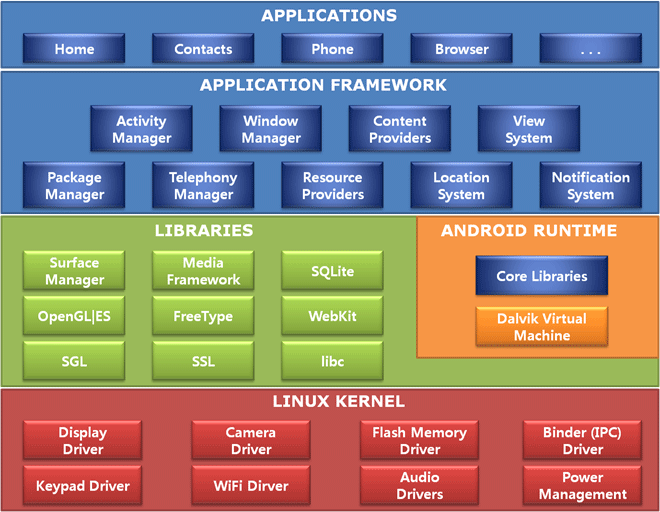
\includegraphics[width=140mm]{external/typical-schematic-of-android_structure.png}} 
\caption{Иллюстрация программного стека Android}
\end{figure}

Далее рассмотрим основные уровни программного стека Android,
изображённые на рисунке \ref{fig:android_arch}:

\textbf{Приложения} : пользовательские приложения, написанные на java,
распространяемые через AndroidMarket или через APK-файлы. Сюда можно
отнести почтовые клиенты, браузеры, медиа-проигрователи и другие
приложения, которыми пользователь обычно пользуется непосредственно
взаимодействуя с ними. 

\textbf{Фреймворк уровня приложений} : набор java классов и пакетов,
предоставляющих API для написания приложений. Набор предоставляемой
функциональности довольно широк: от управления жизненным циклом
приложения до элементов пользовательского интерфейса. Здесь же
предоставляются интерфейсы для взаимодействия приложений друг с другом,
использования одним приложением функций другого.

\textbf{Системные библиотеки} : Набор c/c++ библиотек, применяемых для
написания приложений в Android. Доступны приложениям через фреймворк.
Данные библиотеки реализуют различные ресурсоёмкие задачи, решение
которых посредством java-библиотек вылилось бы в проблемы с
производительностью. В набор входят библиотеки для работы с различными
медиа-форматами (png, jpg, mp3, H.264 и другие), базами данных (sqlite), 
шрифтами, стандартная библиотека с/c++ (Android использует собственную
вариацию под названием bionic), opengl для рисование графики, webkit для
написания web-браузеров. 

\textbf{Android Runtime} : Android использует собственную java-машину
Dalvik Virtual Machine для исполнения java-приложений. DVM используется
из соображений ограниченного объёма памяти на мобильных устройствах. Для
эффективной реализации sandbox-ов для приложений, сущности DVM
запускаются специальным процессом zygote. Также на этом уровне находятся
различные системные сервисы и демоны, работающие с ядром ОС,
устройствами и т.д., например vold, adbd, usbd.

\textbf{Ядро Linux} : В Android используется частично изменённая версия
ядра Linux (обычно используются стабильные ветки ядра 2.6),
оптимизированная под специфику мобильных устройств. Здесь реализуются
драйвера различных физических устройств, системы контроля доступа,
алгоритмы управления виртуальной памятью, файловые системы, сетевой
стек.

В данной работе нас будет интересовать именно ядро Linux. Рассмотрим в
следующем разделе изменения, которые вносит Android в ядро Linux, и на
корелляцию между версиями Linux в Android и в ОС GNU/Linux.

\subsubsection{Сравнения ядер Android и GNU/Linux}

Ядро Linux подходит для использования на самых разных платформах:
встроенные системы, реального времени, высоконагруженные системы и
обычные персональные компьютеры. Когда Linux адаптировался для Android
пришлось вносить изменения в ядро для оптимизации некоторых аспектов
межпроцессного взаимодействия, а также делать поправки на особенности
загрузки ОС на разных устройствах.

Android активно используют передачу данных между процессами, а также
даёт возможность процессам организовать свои процедуры RPC (Remote
Procedure Call). Стандартные средства IPC Linux недостаточно эффективны
для обработки частых запросов на передачу данных, поэтому в Android
появляется существует собственный механизм IPC - Binder. Данный
компонент состоит из нескольких частей: драйвер ядра, реализующий
эффективную передачу данных через общее для всех процессов пространство
ядра, и подсистема рантайма, которая обрабатывает все запросы процессов
на IPC и выполняет их на уровне системных вызовов (взаимодействие с
драйвером).

Система ashmem разделяемой памяти вводит несколько иной, более
эффективный на мобильных устройствах подход, чем классический POSIX SHM.
Вместо файлового API, ashmem позволяет выделять участки разделяемой
памяти с использованием системного вызова mmap, с аргументом файловым
дескриптором, открытым на специальном устройстве /dev/ashmem. Так ashmem
способен отслеживать все области разделяемой памяти в системе, и
уничтожать неиспользуемые в случае нехватки памяти.

В числе прочих изменений, внесённых разработчиками Android можно
упомянуть pmem, аллокатор физической памяти, разделяемой между кодом
ядра и пользовательского пространства, logger реализующий общий
интерфейс логгирования для всех процессов, файловая система yaffs2,
различные патчи, уменьшающие потребление электроэнергии и ещё несколько
архитектурно-зависимых изменений.

По ситуации на март 2014 года, в проекте SEAndroid ядро соответствует 
версии 3.4 обычного ядра Linux.

\subsection{Построение решения}

Рассмотрим возможности для построения системы динамической смены
контекстов безопасности в Android. Для реализации данной задачи
потребуется использовать некоторую систему, позволяющую в зависимости от
внутреннего состояния программы изменять контекст безопасности.
Очевидно, что данная система должна действовать централизованно для всех
приложений в системе, её действия должны быть прозрачны для исполняемого
пользовательского кода. Поэтому предлагается инструментировать
виртуальное адресное пространство приложения контрольными точками, при
попадании исполнения на которые система будет выполнять смену контекста.
Предлагается проводить данную инструментацию при старте приложения из
ядра ОС. На данный момент ОС Android не предоставляет возможности для
динамической инструментации приложения точками останова, но как было
замечено в \ref{subsec:Обзор архитектуры Android} Android использует в
качестве ядра Linux, а значит имеет смысл перенести имеющуюся в Linux
систему динамической инструментации uprobes. 

\subsubsection{uprobes}

Фреймворк динамической инструментации кода приложений точками останова
uprobes используется в системном профилировщике perf для сборки
различной информации по используемым в приложении аппаратным ресурсам,
таким как количество затраченных тактов процессора, количество промахов
кэша при обращении к памяти и прочим аппаратным ресурсам. Нас будет
интересовать непосредственно функциональность uprobes по инструментации
кода точками останова. Uprobes предлагает возможность из кода ядра
регистрировать точки останова в приложениях системы, приложение
идентифицируется по его пути в файловой системе. При каждом запуске
приложения, после того как ядро загрузит в память код приложения, но до
передачи коду возможности исполняться, uprobes подменяет инструкции по
запрошенным адресам на адреса отладочных инструкций, код же оригинальных
инструкций перемещается в специальную область памяти, контролируемую
uprobes. Когда приложение исполняется и попадает на отладочную
инструкцию, то управление передаётся uprobes, а тот уже передаёт его
функции-отладчику, зарегистрированную на обработку данного адреса. Когда
функция-отладчик заканчивает свою работу, uprobes исполняет подменённую
инструкцию и возвращает исполнение на следующую за отлаживаемой
инструкцию. Таким образом отладка происходит прозрачно для приложения.

\subsubsection{Общая схема работы решения}

Предлагается сделать реализацию в виде набора изменений основного ядра
Linux, позволяющих из модулей ядра производить динамическое изменение
контекстов безопасности любых процессов в системе и модуля ядра,
которое, собственно, является наблюдающей системой. 

В наблюдающую систему из пользовательского пространства передается
информация об адресах контрольных точек, информация об изменениях
контекстов безопасности связанных с этими контрольными точками и
информация о том, к какому приложению каждая из точек относится. Вся эта
информация передаётся посредством системных вызовов ioctl, производимых
на специальном устройстве /dev/sad\_droid, которое регистрирует модуль во
время инициализации. Обработчик системного вызова заносит информацию о
смене контекста в целевом приложении в свои внутренние структуры данных
и спомощью uprobes создаёт контрольную точку в приложении.  Устройстве
/dev/sad\_droid будет зарегистрировано в виде обычного символьного устройства.

При попадании контрольного потока на такую точку, uprobes передаст
управлению в наблюдающую систему. Последняя определяет по своим
внутренним структурам новый контекст безопасности для приложения и
производит замену. 

Для переключения контекстов будут использоваться функции SELinux. В ядре
контекст процесса хранится в виде целого числа в специальной структуре
представляющей контекст безопасности текущего потока исполнения.

\begin{comment}
\subsubsection{О ещe одном подходе к выделению
        набора контрольных точек из программы}

В работе~\cite{gornak}
рассматривается средство автоматизации 
построения нормального поведения приложений при помощи
построения автомата безопасности.  Построение 
состояний автомата реализуется при помощи выделения 
блоков кода, соответствующих различным внутренним 
состояниям приложения. 

Тестирование разработанного средства производилось 
на приложении ftpd со следующим набором команд: 

\begin{itemize}
\item DELE -- удалить файл,
\item HELP -- выводит список команд принимаемых сервером,
\item LIST -- возвращает список файлов,
\item NOOP -- пустая операция,
\item QUIT -- отключиться,
\item SYST -- возвращает тип системы,
\item SHOW -- выдать список файлов с описаниями,
\item DESC -- добавить описание файла,
\item TYPE -- установить тип передачи файла (бинарный, текстовый),
\item STOR -- закачать файл,
\item ABOR -- прервать выполнение команды,
\end{itemize}

Основная особенность данного приложения ~--- наличие 
анонимных и авторизованных пользователей. Действия, 
которые разрешено выполнять этим группам пользователей
различаются. 

На рисунке приведен граф потока управления рассматриваемого 
приложения. 

\begin{figure}
 %\centering
  \scalebox{.35}{\begin{tikzpicture}[
    grow=right, 
    level 1/.style={sibling distance=3.5cm,level distance=5.2cm},
    level 2/.style={sibling distance=3.5cm, level distance=6.7cm},
    edge from parent/.style={very thick,draw=blue!40!black!60,
        shorten >=5pt, shorten <=5pt},
    edge from parent path={(\tikzparentnode.east) -- (\tikzchildnode.west)},
    kant/.style={text width=2cm, text centered, sloped},
    every node/.style={text ragged, inner sep=2mm},
    cir/.style={circle, shade, top color=white,
    bottom color=blue!50!black!20, draw=blue!40!black!60, very
    thick },
    cirr/.style={circle, shade, top color=white,
    bottom color=red!50!black!20, draw=red!40!black!60, very
    thick },
    dr/.style={diamond, draw,shade,  top color=white,
    bottom color=red!50!black!20, draw=red!40!black!60, very
    thick},
    bd/.style={draw=blue!50!white, line width=1pt, dash pattern=on 1pt off 4pt on 6pt off 4pt,
                                rectangle, rounded corners},
    d/.style={diamond, draw,shade,  top color=white,
    bottom color=blue!50!black!20, draw=blue!40!black!60, very
    thick},
    bwt/.style = {rectangle, draw,  text width=5em, text centered, minimum height=2em, draw=white, fill=white}]
\node[cir] (1) {};
\node[dr, below of=1, node distance=1.8cm] (if1) {$a^{1}$};
\node[cir, right of=if1, node distance=1.8cm] (exit1) {};
\node[cir, below of=if1, node distance=1.8cm] (203) {};
\node[dr, below of=203, node distance=1.8cm] (while1) {$b^{1}$};
\node[d, below of=while1,  node distance=1.8cm] (if9) {};
\node[d, below of=if9] (if2) {};
\node[cir, below of=if2] (5) {};

\node[d, below of=5] (if3) {};
\node[cir, right of=if3] (607) {};


\node[d, below of=if3] (if4) {};
\node[cir, right of=if4] (8) {};


\node[cir, below of=if4] (9) {};
\node[cirr, below of=9] (55) {$c^{1}$};


\node[cir, below of=55] (10) {};

\node[dr, below of=10, node distance=1.5cm] (if5) {$d^{1}$};
\node[cir, right of=if5, node distance=1.5cm] (12013) {};


\node[cir, below of=if5, node distance=1.5cm] (14) {};

\node[dr, below of=14, node distance=1.9cm] (if6) {$e^{1}$};
\node[cir, right of=if6, node distance=1.5cm] (15016) {};

\node[dr, below of=if6, node distance=1.9cm] (if7) {$f^{1}$};
\node[cir, right of=if7, node distance=1.9cm] (17018) {};

\node[dr, below of=if7, node distance=1.9cm] (if8) {$j^{1}$};
\node[cir, right of=if8, node distance=1.5cm] (19020) {};

\node[cir, below of=if8, node distance=1.5cm] (21) {};

\node[cir, below of=21] (22) {};
\node[cirr, below of=22, node distance=1.5cm] (23) {$h^{2}$};

\node[cirr, below of=23, node distance=1.8cm] (auth) {$k^{2}$};
\node[d, below of=auth, node distance=1.8cm] (if10) {};
\node[cir, right of=if10] (exit24) {};

\node[d, below of=if10] (if11) {};
\node[cir, left of=if11] (return25) {};

\node[d, below of=if11] (if12) {};
\node[cir, right of=if12] (return26) {};
\node[cir, right of=if12, below of=if12] (exit27) {};


\node[d, below of=if12] (if13) {};
\node[bwt, below of=if13, node distance=1cm] (bw) {};

\node[d, left of=bw, node distance=5cm] (while2) {};
\node[d,right of=bw, node distance=5cm] (while3) {};

\node[d, below of=while3] (switch1) {};
\node[cirr, below of=switch1, node distance=1.5cm] (1help) {$l^{2}$};
\node[cirr, left of=1help, node distance=1.5cm] (1add) {$m^{4}$};
\node[cirr, left of=1add, node distance=1.5cm] (1list) {$n^{4}$};
\node[cirr, right of=1help, node distance=1.5cm] (1show) {$o^{4}$};
\node[cirr, right of=1show, node distance=1.5cm] (1desc) {$p^{4}$};
\node[cir, right of=1desc, node distance=1.5cm] (1quit) {};

\node[cir, below of=1help] (1vir) {};

\node[d, below of=while2] (if14) {};

\node[d, below of=if14] (switch2) {};
\node[cirr, below of=switch2, node distance=1.5cm] (2help) {$r^{4}$};
\node[cir, left of=2help, node distance=1.5cm] (2add) {};
\node[cirr, left of=2add, node distance=1.5cm] (2list) {$s^{4}$};
\node[cirr, right of=2help, node distance=1.5cm] (2show) {$t^{2}$};
\node[cir, right of=2show, node distance=1.5cm] (2desc) {};
\node[cir, right of=2desc, node distance=1.5cm] (2quit) {};

\node[cir, below of=2help] (2vir) {};

\draw[->] (1) -- (if1);
\draw[->] (if1) -- (exit1);
\draw[->] (if1) -- (203);
\draw[->] (203) -- (while1);
\draw[->] (while1) -- (if9);

\draw[->] (if9) -- (if2);
\draw[->] (if2) -- (5);
\draw[->] (5) -- (if3);
\draw[->] (if3) -- (if4);
\draw[->] (if4) -- (9);
\draw[->] (9) -- (55);
\draw[->] (55) -- (10);
\draw[->] (10) -- (if5);
\draw[->] (if5) -- (14);
\draw[->] (14) -- (if6);
\draw[->] (if6) -- (if7);

\draw[->] (if7) -- (if8);
\draw[->] (if8) -- (21);



\path (if9) edge[pil,->, bend right=45] node[auto] {} (while1);
\path (9) edge[pil,->, bend left=45] node[auto] {} (while1);

\draw[->] (if3) -- (607);
\draw[->] (607) -- (if4);

\draw[->] (if4) -- (8);
\draw[->] (8) -- (9);

\draw[->] (if5) -- (12013);

\draw[->] (if6) -- (15016);

\draw[->] (if7) -- (17018);

\draw[->] (if8) -- (19020);


\draw[->] (22) -- (23);

\draw[->] (23) -- (auth);
\draw[->] (auth) -- (if10);

\draw[->] (if10) -- (exit24);

\draw[->] (if10) -- (if11);
\draw[->] (if11) -- (return25);

\draw[->] (if11) -- (if12);
\draw[->] (if12) -- (return26);

\draw[->] (if12.south) -- (exit27);

\draw[->] (return26) -- (if13);
\draw[->] (return25) -- (if13);

\draw[->] (if13) -- (while2);
\draw[->] (if13) -- (while3);


\draw[->] (while3) -- (switch1);
\draw[->] (switch1) -- (1help);
\draw[->] (switch1) -- (1add);
\draw[->] (switch1) -- (1list);
\draw[->] (switch1) -- (1show);
\draw[->] (switch1) -- (1desc);
\draw[->] (switch1) -- (1quit);

\draw[->] (1help) -- (1vir);
\draw[->] (1add) -- (1vir);
\draw[->] (1list) -- (1vir);
\draw[->] (1show) -- (1vir);
\draw[->] (1desc) -- (1vir);

\path (1vir) edge[pil,->, bend left=100] node[auto] {} (while3);
\path (if14.west) edge[pil,->, bend left=45] node[auto] {} (while2);


\draw[->] (while2) -- (if14);
\draw[->] (if14) -- (switch2);

\draw[->] (switch2) -- (2help);
\draw[->] (switch2) -- (2add);
\draw[->] (switch2) -- (2list);
\draw[->] (switch2) -- (2show);
\draw[->] (switch2) -- (2desc);
\draw[->] (switch2) -- (2quit);

\draw[->] (2help) -- (2vir);
\draw[->] (2add) -- (2vir);
\draw[->] (2list) -- (2vir);
\draw[->] (2show) -- (2vir);
\draw[->] (2desc) -- (2vir);

\path (2vir) edge[pil,->, bend left=100] node[auto] {} (while2);

\draw[->] (21) -- (22) ;

\node (ifcnf) [bd,  inner sep=2mm, fit = (if1)  (exit1)] {};

\node (whilecnf) [bd,  inner sep=4mm, fit =  (if2) (if3) (if4) (if9) (while1) (5) (607) (8) (9)] {};

\node (if5d) [bd,  inner sep=2mm, fit = (if5) (12013)] {};
\node (if6d) [bd,   inner sep=2mm,fit = (if6) (15016)] {};
\node (if7d) [bd,   inner sep=2mm,fit = (if7) (17018)] {};
\node (if8d) [bd,   inner sep=2mm,fit = (if8) (19020)] {};

\node (2223) [bd,  inner sep=4mm, fit = (22) (23)] {};
\node (auth) [bd,   inner sep=4mm,fit = (auth) (exit24) (return25) (return26) (if10) (if11) (if12) (exit27)] {};

% \draw[->] (switch2) -- (2help);
% \draw[->] (switch2) -- (2add);
% \draw[->] (switch2) -- (2list);
% \draw[->] (switch2) -- (2show);
% \draw[->] (switch2) -- (2desc);
% \draw[->] (switch2) -- (2quit);

\node (switch1d) [bd,   inner sep=4mm,fit = (1help) (1add) (1list) (1show) (1desc) (1quit) (switch1)] {};

\node (switch2d) [bd,   inner sep=4mm,fit = (2help) (2add) (2list) (2show) (2desc) (2quit) (switch2)] {};

\node at (ifcnf.west) [left, inner sep=3mm] {1};
\node at (whilecnf.west) [left, inner sep=3mm] {2};
\node at (if5d.west) [left, inner sep=3mm] {3};
\node at (if6d.west) [left, inner sep=3mm] {4};
\node at (if7d.west) [left, inner sep=3mm] {5};
\node at (if8d.west) [left, inner sep=3mm] {6};
\node at (2223.west) [left, inner sep=3mm] {7};
\node at (auth.west) [left, inner sep=3mm] {8};

\node at (switch1d) [right, inner sep=5cm] {9};
\node at (switch2d) [left, inner sep=5cm] {10};

\end{tikzpicture}
}
  \scalebox{.35}{\begin{tikzpicture}[
    grow=right, 
    level 1/.style={sibling distance=3.5cm,level distance=5.2cm},
    level 2/.style={sibling distance=3.5cm, level distance=6.7cm},
    edge from parent/.style={very thick,draw=blue!40!black!60,
        shorten >=5pt, shorten <=5pt},
    edge from parent path={(\tikzparentnode.east) -- (\tikzchildnode.west)},
    kant/.style={text width=2cm, text centered, sloped},
    every node/.style={text ragged, inner sep=2mm},
    cir/.style={circle, shade, top color=white,
    bottom color=blue!50!black!20, draw=blue!40!black!60, very
    thick },
    cirr/.style={circle, shade, top color=white,
    bottom color=red!50!black!20, draw=red!40!black!60, very
    thick },
    dr/.style={diamond, draw, shade,  top color=white,
    bottom color=red!50!black!20, draw=red!40!black!60, very
    thick},
    bd/.style={draw=blue!50!white, line width=1pt, dash pattern=on 1pt off 4pt on 6pt off 4pt,
                                rectangle, rounded corners},
    d/.style={diamond, draw, shade,  top color=white,
    bottom color=blue!50!black!20, draw=blue!40!black!60, very
    thick},
    bwt/.style = {rectangle, draw,  text width=5em, text centered, minimum height=2em, draw=white, fill=white}]


\node[cir] (1) {};
\node[cirr, below of=1, text width=1mm, node distance=1.8cm] (if1exit1) {$1:a^{1}\ $};
\node[cir, below of=if1exit1, node distance=1.8cm] (203) {};
\node[cirr, below of=203, node distance=1.8cm] (while19) {$2:b^{1}$};
\node[cirr, below of=while19, node distance=1.8cm] (55) {$c^{1}$};


\node[cir, below of=55, node distance=1.8cm] (10) {};

\node[cirr, below of=10, node distance=2cm] (if512013) {$3:d^{1}$};

\node[cir, below of=if512013, node distance=2cm] (14) {};

\node[cirr, below of=14, node distance=2cm] (if615016) {$4:e^{1}$};

\node[cirr, below of=if615016, node distance=2cm] (if717018) {$5:f^{1}$};

\node[cirr, below of=if717018, node distance=2cm] (if819020) {$6:j^{1}$};

\node[cir, below of=if819020, node distance=2cm] (21) {};

\node[cirr, below of=21, node distance=2cm] (2223) {$7:h^{2}$};

\node[cirr, below of=2223, node distance=2cm] (if10252627) {$8:k^{2}$};


\node[d, below of=if10252627, node distance=1.8cm] (if13) {};
\node[bwt, below of=if13, node distance=1.8cm] (bw) {};

\node[d, left of=bw, node distance=2.5cm] (while2) {};
\node[d,right of=bw, node distance=2.5cm] (while3) {};

\node[cirr, below of=while3, node distance=2.5cm] (switch1) {$9:n^{4},m^{4},l^{2},o^{4},p^{4}$};

\node[d, below of=while2, node distance=1.8cm] (if14) {};

\node[cirr, below of=if14, node distance=2cm] (switch2) {$10:s^{4},r^{4},t^{2}$};

\draw[->] (1) -- (if1exit1);
\draw[->] (if1exit1) -- (203);
\draw[->] (203) -- (while19);
\draw[->] (while19) -- (55);
\draw[->] (55) -- (10);
\draw[->] (10) -- (if512013);
\draw[->] (if512013) -- (14);
\draw[->] (14) -- (if615016);
\draw[->] (if615016) -- (if717018);

\draw[->] (if717018) -- (if819020);
\draw[->] (if819020) -- (21);


\draw[->] (21) -- (2223);

\draw[->] (2223) -- (if10252627);
\draw[->] (if10252627) -- (if13);

\draw[->] (if13) -- (while2);
\draw[->] (if13) -- (while3);


\draw[->] (while3) -- (switch1);

\path (switch1) edge[pil,->, bend left=100] node[auto] {} (while3);
\path (if14.west) edge[pil,->, bend left=45] node[auto] {} (while2);


\draw[->] (while2) -- (if14);
\draw[->] (if14) -- (switch2);

\path (switch2) edge[pil,->, bend left=100] node[auto] {} (while2);



\node (12c) [bd,  inner sep=2mm, fit = (1)  (if1exit1) (203) (while19) (55)] {};

\node (3456c) [bd,  inner sep=2mm, fit = (10)  (if512013) (if615016) (14) (21) (if717018) (if819020)] {};
\node (10b) [bd,  inner sep=2mm, fit = (while2)  (if14) (switch2)] {};
\node (9b) [bd,  inner sep=2mm, fit = (switch1) (while3)] {};
% 
% \node (whilecnf) [bd,  inner sep=4mm, fit =  (if2) (if3) (if4) (if9) (while1) (5) (607) (8) (9)] {};
% 
% \node (if5d) [bd,  inner sep=2mm, fit = (if5) (12013)] {};
% \node (if6d) [bd,   inner sep=2mm,fit = (if6) (15016)] {};
% \node (if7d) [bd,   inner sep=2mm,fit = (if7) (17018)] {};
% \node (if8d) [bd,   inner sep=2mm,fit = (if8) (19020)] {};
% 
% \node (2223) [bd,  inner sep=4mm, fit = (22) (23)] {};
% \node (auth) [bd,   inner sep=4mm,fit = (exit24) (return25) (return26) (if10) (if11) (if12) (exit27)] {};
% 
% % \draw[->] (switch2) -- (2help);
% % \draw[->] (switch2) -- (2add);
% % \draw[->] (switch2) -- (2list);
% % \draw[->] (switch2) -- (2show);
% % \draw[->] (switch2) -- (2desc);
% % \draw[->] (switch2) -- (2quit);
% 
% \node (switch1d) [bd,   inner sep=4mm,fit = (1help) (1add) (1list) (1show) (1desc) (1quit) (switch1)] {};
% 
% \node (switch2d) [bd,   inner sep=4mm,fit = (2help) (2add) (2list) (2show) (2desc) (2quit) (switch2)] {};
% 
\node at (12c.west) [left, inner sep=3mm] {12};
\node at (3456c.west) [left, inner sep=3mm] {3456};
\node at (10b.west) [left, inner sep=3mm] {$10^{'}$};
\node at (9b.west) [left, inner sep=3mm] {$9^{'}$};

% \node at (whilecnf.west) [left, inner sep=3mm] {2};
% \node at (if5d.west) [left, inner sep=3mm] {3};
% \node at (if6d.west) [left, inner sep=3mm] {4};
% \node at (if7d.west) [left, inner sep=3mm] {5};
% \node at (if8d.west) [left, inner sep=3mm] {6};
% \node at (2223.west) [left, inner sep=3mm] {7};
% \node at (auth.west) [left, inner sep=3mm] {8};
% 
% \node at (switch1d) [right, inner sep=2.8cm] {9};
% \node at (switch2d) [left, inner sep=3.1cm] {10};

\end{tikzpicture}
}
\caption{Свертка и выделение блоков. Демонстрация шагов алгоритма}
\end{figure}


Итоговое разбиение. Блок 10 соответствует операциям, 
которые может производить анонимный пользователь, 
9 соответствует тем операциям, которые может производить 
авторизованный пользователь.

\begin{figure}
\centering
\scalebox{.80}{\begin{tikzpicture}[
    grow=right, 
    level 1/.style={sibling distance=3.5cm,level distance=5.2cm},
    level 2/.style={sibling distance=3.5cm, level distance=6.7cm},
    edge from parent/.style={very thick,draw=blue!40!black!60,
        shorten >=5pt, shorten <=5pt},
    edge from parent path={(\tikzparentnode.east) -- (\tikzchildnode.west)},
    kant/.style={text width=2cm, text centered, sloped},
    every node/.style={text ragged, inner sep=2mm},
    cir/.style={circle, shade, top color=white,
    bottom color=blue!50!black!20, draw=blue!40!black!60, very
    thick },
    cirr/.style={circle, shade, top color=white,
    bottom color=red!50!black!20, draw=red!40!black!60, very
    thick },
    dr/.style={diamond, top color=white,
    bottom color=red!50!black!20, draw=red!40!black!60, very
    thick},
    bd/.style={draw=blue!50!white, line width=1pt, dash pattern=on 1pt off 4pt on 6pt off 4pt,
                                rectangle, rounded corners},
    d/.style={diamond,  top color=white,
    bottom color=blue!50!black!20, draw=blue!40!black!60, very
    thick},
    bwt/.style = {rectangle, draw,  text width=5em, text centered, minimum height=2em, draw=white, fill=white}]


\node[cirr, node distance=5cm] (1) {$123456:a^{1},b^{1},c^{1},d^{1},e^{1},f^{1},j^{1}$};

\node[cirr, below of=1, node distance=5cm] (3) {$7:h^{2}$};

\node[cirr, below of=3, node distance=3cm] (4) {$8:k^{2}$};

\node[d, below of=4, node distance=3cm] (if) {};

\node[cirr, below of=if, left of=if, node distance=3cm] (10) {$10^{'}:s^{4},r^{4},t^{2}$};

\node[cirr, below of=if, right of=if, node distance=3cm] (9) {$9^{'}:n^{4},m^{4},l^{2},o^{4},p^{4}$};



\draw[->] (1) -- (3);
\draw[->] (3) -- (4);
\draw[->] (4) -- (if);
\draw[->] (if) -- (9);
\draw[->] (if) -- (10);


\end{tikzpicture}
}
\caption{Итоговое разбиение} 
%\label{fig:finalres} 
\end{figure}


На основании полученного разбиения код приложения размечается
контрольными точками. Контрольная точка ставится на входе 
в каждый блок и на выходе из него. Далее работа с этими 
контрольными точками и связанной с ними информацией о смене 
контекстов производится в описанном ниже режиме.
\end{comment}

\begin{comment}
\subsection{Обзор общих принципов работы рассматриваемых 
систем безопасности.} 

\bigskip
\paragraph{SELinux.}

\bigskip
{\bfseries Основные понятия. }

Принудительное присвоение типов (TE). 
И для процессов и для объектов используется 
один и тот же тип атрибутов. Поэтому достаточно 
одной матрицы достаточно для описания доступа к 
взаимодействию между разными типами, при этом 
объекты одного типа могут рассматриваться по-разному, 
если их их ассоциированные классы безопасности 
различны. Пользователи не привязаны к типам 
безопасности напрямую, вместо этого используется RBAC.

Ролевой контроль доступа (RBAC)  используется 
для определения множества ролей, которые могут 
быть назначены пользователям. SELinux расширяет 
модель RBAC до жесткой привязки пользовательских 
ролей к определенным доменам безопасности, роли 
могут быть организованы в виде иерархии приоритетов. 
Такая привязка ролей к доменам позволяет принимать 
большинство решений на основе конфигурации TE. 
Контекст безопасности кроме всего прочего включает 
в себя атрибут роли.

Многоуровневая система безопасности (MLS) 
SELinux предоставляет MLS для случаев, когда есть 
необходимость в традиционной многоуровневой системе 
безопасности. У объектов и субъектов могут быть 
различные уровни и категории. 
Как правило используется лишь один уровень. 

\bigskip
{\bfseries Практический обзор }

Главными элементами системы безопасности 
являются субъект, объект и действия. В классы 
объектов входят классы файлов (blk\_ file, chr\_ 
file, dir, fd,...\ ) ,  классы межпроцессного 
взаимодействия (ipc,msg,msgq,sem,shm), классы 
сетевого взаимодействия (key\_ socket,netif,node,
packet\_ socket,tcp\_ socket), классы объектов 
(passwd), системные классы (capability, process,
Secutity, System). Действия, которые субъекты 
SELinux могут предпринимать над объектами меняются
от класса к классу. Для классов файлов это, например, 
будут создание, исполнение, ссылки, чтение, запись, 
удаление. SELinux ассоциирует атрибуты безопасности 
с субъектами и объектами и основывает свои решения 
на этих атрибутах. Атрибутами являются: идентификатор 
пользователя, роль и тип. Идентификатор пользователя 
— пользовательская учетная запись, ассоциированная с 
субъектом или объектом. У каждого пользователя может 
быть несколько ролей, но в какой-то конкретный момент
времени ему может быть предписана только одна из них. 
Пользователь может менять роли командой newrole. Типы 
(а.к.а. Домены) делят субъекты и объекты на родственные 
группы. Это — главный атрибут безопасности, используемый 
SELinux для принятия решений. Типы позволяют помещать 
процессы в «песочницы» и предотвращать повышение 
привилегий. К примеру, роль суперпользователя - 
sysadm\_ r, его тип — sysadm\_ t. Политика безопасности 
SELinux загружается системой из бинарного файла политики,
который, как правило находится в /etc/security/selinux. 
Бинарная политика собирается при помощи make, исходные 
коды, как правило, находятся в /etc/security/selinux/src/policy.
Инструменты работы с SELinux могут быть разделены на 
три категории: специальные утилиты для настройки и 
использования SELinux, модифицированные версии стандартных 
команд и программ Linux, некоторые добавочные инструменты,
к примеру, для настройки и анализа политик. Среди основных 
команд можно выделить следующие: chcon – помечает файл или 
группу файлов указанным контекстом безопасности, checkpolicy
– позволяет выполнять множество действий, связанных с 
политиками, в том числе, компиляцию политики и ее загрузку 
в ядро; getenforce — позволяет узнать в каком режиме 
работает SELinux, newrole – позволяет пользователю 
перемещаться между ролями; run\_ init — позволяет 
запускать, останавливать или контролировать сервис; 
setenforce позволяет менять режим работы системы; 
setfiles присваивает метки указанной директории и ее 
поддиректориям. Некоторые из измененных программ: cron, 
login, logrotate, pam, ssh. Некоторые инструменты: Apol 
– инструмент для анализа файла policy.conf; SeAudit – 
инструмент для анализа логов, имеющий графический интерфейс; 
SeCmds; SePCuT — инструмент для просмотра и редактирования 
файлов политик; SeUser — модификация пользовательских 
учетных записей. 

\bigskip
{\bfseries Краткий обзор анатомии политики SELinux.}

Файлы политики организованы в виде дерева каталогов, 
корнем которого, как правило, является /etc/security/selinux/src/policy/. 
Основными поддиректориями являются: appconfig 
(определяет дефолтные типы контекстов безопасности); 
domains (определяют домены принудительного присвоения типов); 
file\_contexts (определяют контексты безопасности файлов), 
flask (определяет символы, испльзуемые ядром, совместимым 
с SELinux), macros (определяет макрос М4, используемый в 
исходных текстах политик), tmp (хранит сорцы политик во 
время компиляции), types (определяет несколько главных 
типов, которые не ассоциируются с конкретными доменами). 
Как правило существует два файла, которые определяют домен: 
FC file (file context), определяет контексты безопасности 
директорий и файлов, связанных с данным доменом); TE file 
(type enforcement, определяет вектор правил доступа и 
операций, связанных с доменом). Целью данного обзора не является. 

\bigskip
{\bfseries 5.2. AppArmor.}

AppArmor является системой безопасности, поддерживаемой 
компанией Novell, включена в дистрибутивы openSUSE и SUSE 
Enterprise. В AppArmor для определения того, к каким 
системным ресурсам и с какими привилегиями может 
получить доступ то или иное приложение используются 
политики безопасности (profiles). В отличие от SELinux, 
в которой настройки глобальны для всей системы, профили 
AppArmor разрабатываются индивидуально для каждого 
приложения. Изначально в AppArmor включен набор 
стандартных профилей, запускаемых после установки. 
Отдельно доступны профили для разных популярных программ 
и серверов. Кроме этого существуют инструменты для генерации 
профилей (genprof и logprof). Основная идея — верный выбор 
приложений, нуждающихся в ограничении привилегий и 
создание/редактирование профилей безопасности. Таким 
образом, в случае эксплойта, нанесенный ущерб сводится 
к минимуму. Система может работать в двух режимах: режиме 
обучения (complain) и в принудительном режиме (enforce). 
В первом из них все нарушения правил профиля разрешены, 
но немедленно регистрируются. Загрузка профиля в 
принудительном режиме предписывает системе отправлять 
сообщения о нарушениях в syslogd. Запуск и остановку 
AppArmor можно осуществлять при помощи команды rcapparmor 
с одним из следующих параметров: start (загрузка модуля 
ядра, анализ профиля, монтирование своей фс); stop (фс 
размонтируется, профили становятся недействительными); 
reload (перезагрузка профилей), status (информация о 
количестве запущенных профилей, в каком режиме они 
работают). Инструменты командной строки AppArmor: autodep 
(создает приблизительный профиль для программы или 
рассматриваемого приложения); complain (устанавливает 
профиль AppArmor в обучающий режим); enforce (переводит 
профиль в принудительный режим); genprof (генерирует профиль,
программа указывается при запуске); logprof (управляет
профилями AppArmor); unconfined (выводит список процессов 
с портами tcp и udp, которые не имеют загруженных 
профилей AppArmor). Система AppArmor построена на системе 
полных путей к файлам, проще говоря, типичное описание 
профиля выглядит примерно так: 

\bigskip
\begin{flushleft}
\texttt{\#include <tunables/global> \\  
/usr/bin/man { \\ 
	\#include <abstractions/base> \\
	\#include <abstractions/nameservice> \\
	capability setgid, \\
	capability setuid, \\
	/usr/lib/man-db/man Px,}\\ 
}
{\sloppy

}
\end{flushleft}

\bigskip
Профиль состоит из файлов, каталогов с указанием полных 
путей к ним и прав доступа к этим объектам. При этом r — 
разрешение на чтение, w — запись(за исключением создания 
и удаления файлов), ix — исполнение и наследование текущего 
профиля, px — исполнение под специфическим профилем, Px — 
защищенное выполнение, ux — неограниченное исполнение, 
Ux — защищенное неограниченное исполнение, m — присвоение 
участку памяти атрибута «исполняемый», I — жесткая ссылка. 
Чтобы подключить готовый профиль к AppArmor, достаточно его 
скопировать в каталог /etc/apparmor.d. 

\bigskip
{\bfseries PaX }

Основная цель данного проекта — изучение различных защитных 
механизмов, защищающих от эксплойтов уязвимостей ПО, которые 
предоставляют злоумышленнику полные права на чтение/запись в 
системе. Исполнение кода связано с необходимостью изменять 
ход выполнения процесса используя уже существующий код. Одна 
из основных проблем — подмена адресов возврата из функций и 
подмена самих адресов функций. Для установки PaX требуется 
наложить патч на дерево исходных кодов ядра, после чего собрать 
ядро и установить в систему. 

\bigskip
{\bfseries Trusted BSD.}

Проект TrustedBSD – проект разработки расширения существующей системы 
безопасности FreeBSD, включая расширенные атрибуты UFS2, 
списки контроля доступа, OpenPAM, аудит событий 
безопасности с OpenBSM, мандатное управление доступом 
и TrustedBSD MAC Framework. Trusted BSD была задумана 
как система, удовлетворяющая стандартам «оранжевой книги». 
Расширенные атрибуты UFS2 позволяют ядру и 
пользовательским процессам помечать файлы 
именованными метками. Это предоставляет место для 
хранение данные, необходимые системе безопасности, 
такие, как ACL и метки MAC. Списки контроля доступа 
— расширения дискреционного контроля доступа. Аудит 
системных событий позволяет вести избирательный 
логгинг важных системных событий для последующего 
анализа, обнаружения вторжений, и мониторинга в 
реальном времени. Начиная с версии 5.0 в ядре FreeBSD 
появилась поддержка MAC Framework, прошедшая испытания 
в TrustedBSD. Данный фреймворк позволяет создавать политики, 
определяющие принудительное присвоение доменов и типов (DTE), 
многоуровневую систему безопасности (MLS). Данный фреймворк 
предоставляет интерфейсы управления фреймворком, примитивы 
для синхронизации, механизм регистрации политик, примитивы 
для разметки объектов системы, разные политики, 
реализованные в виде модулей политики MAC и набор 
системных вызовов для приложений. При регистрации 
политики, происходит регистрация специальной структуры 
(struct mac\_policy\_ops), содержащей функции MAC 
framework, реализуемые политикой. На данный момент 
существуют следующие политики: 

mac\_biba – Реализация политики Biba, во многом 
схожей с MLS. Позволяет присваивать объектам и 
субъектам системы атрибуты доступа, которые образую 
иерархию уровней. Все операции над информацией в 
системе контролируются исходя из уровней 
взаимодействующих сущностей. 

mac\_ifoff позволяет администраторам контролировать 
сетевой трафик. 

mac\_lomac (Low-watermark MAC) еще одна 
реализация многоуровневого контроля доступа. 

mac\_bsdextended (file system firewall ) Система 
защиты файлов, основанная на определении прав 
доступа на основании роли пользователя. 

mac\_mls~--- реализация политики MLS. Объекты 
классифицируются  некоторым образом, субъектам 
присваивают уровень доступа. 

\bigskip
{\bfseries ОС «Феникс».}

ОС «Феникс» является отечественной разработкой — 
разработка СпбГУ, целью которой является создание 
специальной защищенной операционной системы класса 
Unix, отвечающей отечественным требованиям и 
стандартам информационной безопасности. «Феникс» 
представляет собой микроядерную, многопользовательскую, 
многозадачную, многопоточную операционную систему класса 
UNIX со встроенными механизмами защиты, 
обеспечивающими контроль взаимодействий, управление 
доступом, контроль целостности, 
идентификацию/аутентификацию пользователей 
и возможность подключения средств шифрования. 
Микроядерная архитектура отвечает принципу 
интегрированности, поскольку только в микроядерных 
системах для взаимодействий используется 
единственный способ — обмен сообщениями. 
Контроль доступа органично встраивается в этот 
механизм, причем, установив тотальный контроль 
над потоками сообщений, можно быть уверенным в 
том, что контролируются все взаимодействия в системе.
Принцип инвариантности определил организацию всех 
взаимодействий в «Феникс» на основе архитектуры 
клиент-сервер. В соответствии с принципом унификации 
доступ к объектам в «Феникс» осуществляется через 
Унифицированный Интерфейс Доступа к Объектам (УНИДО), 
определяющий множество операций, универсальных для 
всех типов объектов, в виде универсального набора 
методов, позволяющего выполнять все операции доступа к 
объектам, их создания и уничтожения, управления их
свойствами. Использование УНИДО единственный способ 
выполнения операций над объектами в «Феникс». 
Интерфейс оформлен в виде абстрактного класса, от 
которого наследуются интерфейсы всех серверов «Феникс», 
реализуемых УНИДО. Наличие набора типовых операций 
упрощает реализацию контроля доступа, поскольку 
определено однозначное соответствие между методами 
УНИДО и операциями доступа, описываемыми моделями 
безопасности. 

\bigskip
{\bfseries Vista Kernel-Mode Security.}

В ОС Windows Vista была расширена модель 
безопасности, присутствовавшая в предыдущих 
версиях системы(вплоть до XP SP2). Среди 
нововведений стоит отметить цифровые подписи 
драйверов, PatchGuard, Kernel-mode Code 
Integrity Checks, optional support for Secure 
Bootup using a TPM hardware chip, restricred 
user-mode access to \\ Device\\ PhysicalMemory. 

\bigskip
{\bfseries Driver Signing }. Анализируя эксплойты 
уязвимостей прошлых версий ОС, мы можем 
прийти к выводу, что наиболее распространенный 
способ, используемый вредоносным кодом для 
проникновения в ядро — проникновение через 
драйверы. Поэтому Vista не только требует подписи 
от драйвера, но и требует подпись именно от одного 
из восьми доверенных сертификатов. 

\bigskip
{\bfseries PatchGuard} был разработан для предотвращения 
патчей ядра ОС Виста х64. Защищает ядро путем периодической 
проверки на валидность некоторых структур данных и образов 
системы. PatchGuard кроется в NTOSKRNL.EXE и проверяет особо 
критичные системные структуры через случайные промежутки 
времени, обычно порядка 5-10 минут. Если была обнаружена 
модификация, «system will blue screen with the following 
bugcheck(which will obviously cause the user to lose all 
unsaved data)». (возможно ли обнаружить и убить тред 
PatchGuard?) 

\bigskip
Disabling \\Device\\PhysivalMemory 
Отказ от возможности доступа к Disabling \\ Device\\ PhysivalMemory 
из пользовательского пространства тоже является 
серьезным шагом на пути предотвращения доступа вредоносного кода к ядру. 

\bigskip
{\bfseries Code Integrity (CI.DLL) }
Импортируется статически NTOSKRNL. Защищает систему 
тем, что проверяет  системные исполняемые файлы на 
наличие изменений, в том числе и из-за внедрения 
вредоносного кода, наличие в системе неподписанных 
драйверов, запущенных в режиме ядра. В чем же отличие 
CI от PatchGuard, если они предоставляют схожую 
функциональность? CI может быть отключен, если 
отключены integrity checks, PatchGuard всегда включен. 
Кроме этого, эти методы разрабатывались разными 
командами внутри Microsoft и по заявлениям 
разработчиков, служат разным целям. 

\bigskip
{\bfseries Возможные направления атак. }
Kernel-Mode Network Drivers. 
Виста поддерживает некоторые сетевые протоколы 
в виде драйверов уровня ядра. Если уязвимость 
обнаружена в одном их этих подписанных драйверах, 
это бы дало возможность заполучить удаленный 
контроль над всей машиной. 

Disabling Driver Signing and Code Integrity 

Самый простой путь преодоления всех сложностей, 
связанных с подписями драйверов — патч исполняемых 
файлов и отключение проверок подписей вообще. 
Для загрузки неподписанных драйверов во время 
выполнения NTOSKRNL.EXE должен быть пропатчен. 
Но, патч ядра несет угрозу его цифровой подписи, 
следовательно, WINLOAD.EXE откажется загружать ядро.

\bigskip
{\bfseries Apple Seatbelt. }

Кроме возможности использования интерфейсов 
при программировании, позволяет помещать приложения 
в «песочницу», где их поведение будет контролироваться 
на основании определенных профилей. Данные профили 
находятся в /usr/share/sandbox и состоят из 
allow/deny определений и регулярных выражений 
для определения прав доступа к ресурсам системы. 
Объекты определяются по абсолютному пути (POSIX). 
Пример конфигурационного файла: 

\begin{flushleft}
\bigskip
\texttt{(version1)\\
(debug deny)\\
(allow default)\\
(allow process*)\\
(deny network-outbound)\\
(allow file-read-data file-read-metadata\\
(regex "\^ /.*"))\\
(deny file-write* \\
(regex "\^ /.*"))\\
(allow file-write*\\
(regex "\^ /Users/johndoe/Library/Preferences.*"))\\
(allow file-write* file-read-data file-read-metadata\\
(regex "\^ (/private)?/tmp/"))\\
(import "bsd.sb")
}
\bigskip
\end{flushleft}

Помещение в «песочницу» приложения на Cocoa производится следующим образом:
\% sandbox-exec -n localonly /Applications/TextEdit.app /Contents/MacOS/TextEdit

\end{comment}

\newpage
\section{Описание практической части}

В разделе \ref{issled} были определены подзадачи,
которые нужно решить:
\begin{itemize}

\item Внесение изменений в ядро Linux для поддержки динамического
        изменения контекстов наблюдаемых приложений

\item Реализация поддержки установки контрольных точек в наблюдаемое
        приложение

\item Реализация поддержки наблюдения за определенными событиями в
        ядре Linux

\item Реализация возможности конфигурации из пользовательского
        пространства
        
\end{itemize}

В следуюхих разделах описаны решения каждой из подзадач и итоговая
схема решения.

\subsection{Общая схема работы решения}

Решение организовано в виде набора изменений основного ядра Linux,
позволяющих из модулей ядра производить динамическое изменение
контекстов безопасности любых процессов в системе и модуля
ядра, которое, собственно, является наблюдающей системой.

В наблюдающую систему из пользовательского пространства передается
информация об адресах контрольных точек, информация об изменениях
контекстов безопасности связанных с этими контрольными
точками и информация о том, к какому приложению каждая из точек относится.

Далее, в процессе работы система отслеживает все порождения новых процессов
в системе. Если у системы имеется информация относительно необходимости
установки контрольных точек в данный процесс, она производит установку
контрольных точек и начинает наблюдение за ходом исполнения данного процесса.

\subsection{Поддержка динамического изменения контекстов приложений
            в ядре Linux}

Ядро Linux не предоставляет возможность динамически изменять
контексты безопасности приложений из модулей ядра. При этом
ядро хранит в своей памяти матрицу доступа, определяемую
политикой безопаности SELinux. Все операции, связанные с
данной матрицей доступа, выполняются соответствующей подсистемой
ядра, реализованной в ./security/selinux/. Данная подсистема,
в частности, использует набор интерфейсов LSM для применения
описанной политики безопасности SELinux.

Все контексты безопасности, описанные в рамках политики SELinux
однозначно отображаются на конечное подмножество натуральных чисел,
ограниченное сверху общим числом контекстов, присутствующих в
данной политике. В служебных структурах ядра, описывающих процесс,
контекст безопасности SELinux относящийся к данному процессу
представлен целым числом. В подсистеме ядра, реализующей SELinux
присутствуют методы, производящие преобразования строковых
представлений контекстов безопасности в соответствующие им
натуральные числа и обратно.

\lstinputlisting[label=samplecode1,caption=Листинг 1]{sourceCode/exports1.c}

Для того, чтобы предоставить модулям ядра возможность использовать
данные методы, определяются экспортируемые из основного ядра функции,
являющиеся обёрткой для приведенных выше функций. Определение
экспортируемых методов производится в файле ./security/selinux/exports.c.
Пример для функции, преобразующей строковое представление контекста
безопасности к беззнаковому числу.

\lstinputlisting[label=samplecode2,caption=Экспортируемые функции преобразования контекстов]{sourceCode/exports2.c}

Преобразование контекста безопасности процесса в подсистеме ядра SELinux
осуществляется методами security\_kern\_setprocattr и
security\_kern\_getprocattr. Для них необходимо определить
экспортируемые методы аналогично приведенным выше. Пример для
security\_kern\_setprocattr:

\lstinputlisting[label=samplecode2,caption=Экспортируемые функции изменения контекстов процессов]{sourceCode/exports3.c}

Кроме того, методы security\_kern\_setprocattr и
security\_kern\_getprocattr могут работать лишь с тем процессом,
который в данный момет является исполняемым(FIXME). В данные методы
вносятся изменения, позволяющие изменение контекстов любых процессов
в системе.

\subsection{Реализация установки контрольных точек в наблюдаемое
            приложение}


Как было сказано ранее, под контрольной точкой в данной работе
понимается адрес сегменте кода наблюдаемого приложения.
Для установки и наблюдения за попаданием исполнения на
контрольные точки были выбраны подсистемы ядра utrace-uprobes.
Данные подсистемы позволяют модулям ядра Linux выступать в
роли отладчиков пользовательских приложений, в том числе и
устанавливать в адресном пространстве наблюдаемых приложений
точки останова и обрабатывать события <<попадания>> исполнения
на эти точки.

Подсистема utrace предоставляет средства создания 
отладчиков в виде модулей ядра, в то время, как 
uprobes использует utrace для установки точек 
останова в сегменте кода процесса и наблюдения за попаданием 
исполнения на них. 

Рассмотрим особенности использования этой системы 
более подробно. Как было сказано выше, utrace является подсистемой 
ядра, позволяющей создавать отладчики, работающие в 
пространстве ядра в виде модулей. При этом, модуль 
должен реализовать некоторые функции-обработчики 
событий, происходящих в отлаживаемом приложении. 

Пример:

\lstinputlisting[label=samplecode2,caption=Экспортируемые функции изменения контекстов процессов]{sourceCode/utrace1.c}

\bigskip
Как только отлаживаемый процесс совершит системный вызов, будет вызвана 
соответствующая функция отлаживаемого движка - {\texttt report\_sysc
all\_entry()} (разумеется, если она была зарегистрирована). Вызов 
данного обработчика происходит до выполнения системного вызова, 
отладчик может безопасно получать доступ к остановленному отлаживаемому 
процессу. Функция-обработчик возвращает битовую маску, которая определяет, что 
должно произойти далее~--- можно изменять состояние отладки, 
прекращать отладку, скрывать событие от других отладочных 
движков и многое другое. 

Отладочный движок регистрируется следующей функцией: 

\lstinputlisting[label=samplecode2,caption=Экспортируемые функции изменения контекстов процессов]{sourceCode/utrace2.c}

\bigskip 
Данный вызов ассоциирует отладочный движок к указанным процессом. 
Возможна регистрация более чем одного отладочного движка для 
одного и того же процесса~--- серьезное отличие от ptrace(). 
Только что зарегистрированный движок ничего не делает и 
находится в состоянии idle. Для запуска необходимо указать 
соответствующие флаги в вызове функции 

\lstinputlisting[label=samplecode2,caption=Экспортируемые функции изменения контекстов процессов]{sourceCode/utrace3.c}

\bigskip 
Существует специальный флаг - {\texttt UTRACE\_EVENT(QUIESCE)}, 
который может переключать процесс в состояние ожидания. В общем 
случае, все операции с процессом в первую очередь требуют 
установки этого флага, после чего можно ожидать исполнения 
коллбека {\texttt report\_quiesce()}, который извещает об 
остановке процесса. Есть множество других событий, извещения 
о которых могут быть получены отладочным движком. В их числе 
fork(), exec(), получение сигнала, завершение процесса, вызов 
системного вызова и др..

\bigskip
{\bfseries Uprobes.}

\bigskip
Uprobes является клиентом системы utrace и входит в состав утилит для 
наблюдения за событиями в системе Systemtap в качестве модуля ядра. 
Кроме этого, существуют патчи, позволяющие интегрировать uprobes 
непосредственно в ядро Linux. Основной функцией данного набора функций 
является обеспечение возможности проставления контрольных точек в код 
отлаживаемого процесса и регистрация функций, обрабатывающих события, 
связанные с данными точками. Есть два типа таких контрольных точек: 
uprobes и uretprobes. 

Контрольная точка типа Uprobe может быть установлена на любой адрес в 
виртуальном адресном пространстве процесса и сработает при попадании 
исполнения на инструкцию, расположенную по этому адресу. Контрольная
точка типа uretprobe сработает при завершении работы указанной функции
в отлаживаемом процессе. При регистрации точки останова, uprobes сохраняет
копию инструкции, расположенной по этому адресу в приложении, останавливает 
его исполнение, подменяет первые байты по этому адресу на инструкцию 
точки останова (int3 на i386 x86\_64) и вновь запускает исполняемое 
приложение. Когда исполнение попадает на эту инструкцию, срабатывает 
ловушка и генерируестя сигнал SIGTRAP.

Uprobes получает этот сигнал и 
находит связанную с ним точку останова и ее функцию-обработчик. 
Отлаживаемый процесс будет остановлен до завершения работы 
функции-обработчика. После завершения работы функции-обработчика uprobes 
исполняет сохраненную команду, которая первоначально располагалась 
по адресу точки останова в пользовательском процессе и вновь запускает 
пользовательский процесс.   

Регистрация контрольной точки может быть произведена с помощью функции
 
\lstinputlisting[label=samplecode2,caption=Экспортируемые функции изменения
                                контекстов процессов]{sourceCode/uprobes1.c}

Будет установлена точка останова в виртуальном адресном пространстве 
процесса u->pid по адресу u->vaddr и с обработчиком v->handler, который
 может быть определен следующим образом: 

\lstinputlisting[label=samplecode2,caption=Экспортируемые функции изменения
                                контекстов процессов]{sourceCode/uprobes2.c}

При завершении отлаживаемого процесса, либо при вызове функции exec() 
uprobes автоматически удаляет все контрольные точки и их обработчики. 
При выполнении вызова fork() во вновь созданном процессе удаляются все 
контрольные точки. 

\subsection{Наблюдение за определенными событиями в системе}

Как было сказано в общей схеме работы решения, в контролирующей
системе необходимо получать уведомления о различных событиях в
ядре. В частности, о порождении определенных процессов.
Порождение новых процессов в Linux производится с помощью
примитивов fork()/exec(). Для определения того, что был запущен
интересующий нас процесс, необходимо проанализировать параметры
системного вызова execve.

В ядре Linux отсутствуют стандартные интерфейсы для сбора
информации о системных вызовах и их параметрах.
Реализуемая система должна получать такую информацию самостоятельно.

Для этого используется подсистема kprobes, которая
позволяет устанавливать точки останова на любую экспортируемую из
основного ядра функцию. Точка останова ставится на выход из обработки
системного вызова execve, что позволяет контролирующей системе получать
информацию обо всех системных вызовах execve, происходящих в системе.
Анализ параметров данного системного вызова и возвращаемого им значения
позволяет получать информацию обо всех порожденных процессах, вызвавших
функцию execve после своего создания.

\subsection{Реализация возможности конфигурации из пользовательского пространства}
\label{contpoints}

Стандартным методом взаимодействия пространства ядра с пользовательскими
приложениями является интерфейс ioctl. Приложения пользовательского
пространства имеют возможность производить конфигурацию реализованной
системы с помощью данного интерфейса. Для этого в ядро передаются
структуры, содержащие информацию о пути до исполняемого файла, адрес
в виртуальном адресном пространстве процесса и символьное представление
нового контекста безопасности:

\lstinputlisting[label=samplecode2,caption=Экспортируемые функции изменения
                                контекстов процессов]{sourceCode/apathy1.c}

Данная структура содержит в себе информацию о том, что при запуске
указанного исполнимого файла в результирующем процессе по указанному
адресу необходимо разместить контрольную точку. При попадании
исполнения на эту контрольную точку для данного процесса необходимо
произвести изменение контекста безопасности на указанное в данной структуре.

Информация, сообщённая наблюдающему модулю ядра хранится в его памяти
и используется всякий раз, когда запускается процесс, за которым необходимо
установить наблюдение.

\subsection{Тестирование реализации на модельном примере приложения,
                содержащего уязвимость}

В мае 2011 года была обнаружена уязвимость в почтовом сервере
exim4, позволяющая удалённому атакующему получить доступ к конфиденциальной
информации, хранящейся на сервере. Атаки на данную уязвимость не могут
быть предотвращены стандартной реализацией SELinux.

Работоспособность разработанной системы было решено продемонстрировать
на модельном примере, содержащим уязвимость, аналогичную реальному приложению.

%% ===========================================================================
\begin{comment}

\subsection{Выделение некоторого набора адресов 
		контрольных точек из программы}

Контрольной точкой является некоторый адрес 
в виртуальном адресном пространстве процесса.
Попадание исполнения на контрольную точку 
сигнализирует наблюдающей системе об изменении 
внутреннего состояния наблюдаемого процесса. 

Ставится задача определения адресов контрольных точек 
в наблюдаемом процессе. 

В работе прошлого года предполагалось выделение 
контрольных точек при наличии исходных текстов 
наблюдаемого приложения на языках C/C++ и
информации о том, 
с какими параметрами приложение было собрано.
На этапе подготовки экспертом расставляются 
контрольные точки в исходных текстах приложения. 
При сборке адреса данных контрольных точек 
компонуются в отдельную секцию в исполняемом 
файле приложения. 

Данные адреса связываются с определенной информацией 
в текстовом формате, которая описывается в конфигурационном файле.
Информация, описанная в конфигурационном файле 
определяет работу наблюдающей системы.

В этом году было решено добавить возможность работы 
без необходимости в исходных текстах наблюдаемого 
приложения, а также без необходимости пересборки 
и добавления новой секции с адресами в исполняемый 
файл приложения.

Данный подход позволяет расширить класс приложений, 
наблюдение за поведением которых возможно, до всех 
приложений, работающих в нативном коде. Кроме этого, 
наличие исходных текстов наблюдаемых приложений 
перестает быть необходимым условием.

\subsection{О еще одном подходе к разделению внутренних пространств 
		состояний приложения}
\bigskip 
В работе~\cite{gornak} рассматривается средство автоматизации 
построения нормального поведения приложений при помощи
построения автомата безопасности.  Построение 
состояний автомата реализуется при помощи выделения 
блоков кода, соответствующих различным внутренним 
состояниям приложения. 

Тестирование разработанного средства производилось 
на приложении ftpd со следующим набором команд: 

\begin{itemize}
\item DELE -- удалить файл,
\item HELP -- выводит список команд принимаемых сервером,
\item LIST -- возвращает список файлов,
\item NOOP -- пустая операция,
\item QUIT -- отключиться,
\item SYST -- возвращает тип системы,
\item SHOW -- выдать список файлов с описаниями,
\item DESC -- добавить описание файла,
\item TYPE -- установить тип передачи файла (бинарный, текстовый),
\item STOR -- закачать файл,
\item ABOR -- прервать выполнение команды,
\end{itemize}

Основная особенность данного приложения ~--- наличие 
анонимных и авторизованных пользователей. Действия, 
которые разрешено выполнять этим группам пользователей
различаются. 

На рисунке приведен граф потока управления рассматриваемого 
приложения. 

\begin{figure}
 %\centering
  \scalebox{.35}{\begin{tikzpicture}[
    grow=right, 
    level 1/.style={sibling distance=3.5cm,level distance=5.2cm},
    level 2/.style={sibling distance=3.5cm, level distance=6.7cm},
    edge from parent/.style={very thick,draw=blue!40!black!60,
        shorten >=5pt, shorten <=5pt},
    edge from parent path={(\tikzparentnode.east) -- (\tikzchildnode.west)},
    kant/.style={text width=2cm, text centered, sloped},
    every node/.style={text ragged, inner sep=2mm},
    cir/.style={circle, shade, top color=white,
    bottom color=blue!50!black!20, draw=blue!40!black!60, very
    thick },
    cirr/.style={circle, shade, top color=white,
    bottom color=red!50!black!20, draw=red!40!black!60, very
    thick },
    dr/.style={diamond, draw,shade,  top color=white,
    bottom color=red!50!black!20, draw=red!40!black!60, very
    thick},
    bd/.style={draw=blue!50!white, line width=1pt, dash pattern=on 1pt off 4pt on 6pt off 4pt,
                                rectangle, rounded corners},
    d/.style={diamond, draw,shade,  top color=white,
    bottom color=blue!50!black!20, draw=blue!40!black!60, very
    thick},
    bwt/.style = {rectangle, draw,  text width=5em, text centered, minimum height=2em, draw=white, fill=white}]
\node[cir] (1) {};
\node[dr, below of=1, node distance=1.8cm] (if1) {$a^{1}$};
\node[cir, right of=if1, node distance=1.8cm] (exit1) {};
\node[cir, below of=if1, node distance=1.8cm] (203) {};
\node[dr, below of=203, node distance=1.8cm] (while1) {$b^{1}$};
\node[d, below of=while1,  node distance=1.8cm] (if9) {};
\node[d, below of=if9] (if2) {};
\node[cir, below of=if2] (5) {};

\node[d, below of=5] (if3) {};
\node[cir, right of=if3] (607) {};


\node[d, below of=if3] (if4) {};
\node[cir, right of=if4] (8) {};


\node[cir, below of=if4] (9) {};
\node[cirr, below of=9] (55) {$c^{1}$};


\node[cir, below of=55] (10) {};

\node[dr, below of=10, node distance=1.5cm] (if5) {$d^{1}$};
\node[cir, right of=if5, node distance=1.5cm] (12013) {};


\node[cir, below of=if5, node distance=1.5cm] (14) {};

\node[dr, below of=14, node distance=1.9cm] (if6) {$e^{1}$};
\node[cir, right of=if6, node distance=1.5cm] (15016) {};

\node[dr, below of=if6, node distance=1.9cm] (if7) {$f^{1}$};
\node[cir, right of=if7, node distance=1.9cm] (17018) {};

\node[dr, below of=if7, node distance=1.9cm] (if8) {$j^{1}$};
\node[cir, right of=if8, node distance=1.5cm] (19020) {};

\node[cir, below of=if8, node distance=1.5cm] (21) {};

\node[cir, below of=21] (22) {};
\node[cirr, below of=22, node distance=1.5cm] (23) {$h^{2}$};

\node[cirr, below of=23, node distance=1.8cm] (auth) {$k^{2}$};
\node[d, below of=auth, node distance=1.8cm] (if10) {};
\node[cir, right of=if10] (exit24) {};

\node[d, below of=if10] (if11) {};
\node[cir, left of=if11] (return25) {};

\node[d, below of=if11] (if12) {};
\node[cir, right of=if12] (return26) {};
\node[cir, right of=if12, below of=if12] (exit27) {};


\node[d, below of=if12] (if13) {};
\node[bwt, below of=if13, node distance=1cm] (bw) {};

\node[d, left of=bw, node distance=5cm] (while2) {};
\node[d,right of=bw, node distance=5cm] (while3) {};

\node[d, below of=while3] (switch1) {};
\node[cirr, below of=switch1, node distance=1.5cm] (1help) {$l^{2}$};
\node[cirr, left of=1help, node distance=1.5cm] (1add) {$m^{4}$};
\node[cirr, left of=1add, node distance=1.5cm] (1list) {$n^{4}$};
\node[cirr, right of=1help, node distance=1.5cm] (1show) {$o^{4}$};
\node[cirr, right of=1show, node distance=1.5cm] (1desc) {$p^{4}$};
\node[cir, right of=1desc, node distance=1.5cm] (1quit) {};

\node[cir, below of=1help] (1vir) {};

\node[d, below of=while2] (if14) {};

\node[d, below of=if14] (switch2) {};
\node[cirr, below of=switch2, node distance=1.5cm] (2help) {$r^{4}$};
\node[cir, left of=2help, node distance=1.5cm] (2add) {};
\node[cirr, left of=2add, node distance=1.5cm] (2list) {$s^{4}$};
\node[cirr, right of=2help, node distance=1.5cm] (2show) {$t^{2}$};
\node[cir, right of=2show, node distance=1.5cm] (2desc) {};
\node[cir, right of=2desc, node distance=1.5cm] (2quit) {};

\node[cir, below of=2help] (2vir) {};

\draw[->] (1) -- (if1);
\draw[->] (if1) -- (exit1);
\draw[->] (if1) -- (203);
\draw[->] (203) -- (while1);
\draw[->] (while1) -- (if9);

\draw[->] (if9) -- (if2);
\draw[->] (if2) -- (5);
\draw[->] (5) -- (if3);
\draw[->] (if3) -- (if4);
\draw[->] (if4) -- (9);
\draw[->] (9) -- (55);
\draw[->] (55) -- (10);
\draw[->] (10) -- (if5);
\draw[->] (if5) -- (14);
\draw[->] (14) -- (if6);
\draw[->] (if6) -- (if7);

\draw[->] (if7) -- (if8);
\draw[->] (if8) -- (21);



\path (if9) edge[pil,->, bend right=45] node[auto] {} (while1);
\path (9) edge[pil,->, bend left=45] node[auto] {} (while1);

\draw[->] (if3) -- (607);
\draw[->] (607) -- (if4);

\draw[->] (if4) -- (8);
\draw[->] (8) -- (9);

\draw[->] (if5) -- (12013);

\draw[->] (if6) -- (15016);

\draw[->] (if7) -- (17018);

\draw[->] (if8) -- (19020);


\draw[->] (22) -- (23);

\draw[->] (23) -- (auth);
\draw[->] (auth) -- (if10);

\draw[->] (if10) -- (exit24);

\draw[->] (if10) -- (if11);
\draw[->] (if11) -- (return25);

\draw[->] (if11) -- (if12);
\draw[->] (if12) -- (return26);

\draw[->] (if12.south) -- (exit27);

\draw[->] (return26) -- (if13);
\draw[->] (return25) -- (if13);

\draw[->] (if13) -- (while2);
\draw[->] (if13) -- (while3);


\draw[->] (while3) -- (switch1);
\draw[->] (switch1) -- (1help);
\draw[->] (switch1) -- (1add);
\draw[->] (switch1) -- (1list);
\draw[->] (switch1) -- (1show);
\draw[->] (switch1) -- (1desc);
\draw[->] (switch1) -- (1quit);

\draw[->] (1help) -- (1vir);
\draw[->] (1add) -- (1vir);
\draw[->] (1list) -- (1vir);
\draw[->] (1show) -- (1vir);
\draw[->] (1desc) -- (1vir);

\path (1vir) edge[pil,->, bend left=100] node[auto] {} (while3);
\path (if14.west) edge[pil,->, bend left=45] node[auto] {} (while2);


\draw[->] (while2) -- (if14);
\draw[->] (if14) -- (switch2);

\draw[->] (switch2) -- (2help);
\draw[->] (switch2) -- (2add);
\draw[->] (switch2) -- (2list);
\draw[->] (switch2) -- (2show);
\draw[->] (switch2) -- (2desc);
\draw[->] (switch2) -- (2quit);

\draw[->] (2help) -- (2vir);
\draw[->] (2add) -- (2vir);
\draw[->] (2list) -- (2vir);
\draw[->] (2show) -- (2vir);
\draw[->] (2desc) -- (2vir);

\path (2vir) edge[pil,->, bend left=100] node[auto] {} (while2);

\draw[->] (21) -- (22) ;

\node (ifcnf) [bd,  inner sep=2mm, fit = (if1)  (exit1)] {};

\node (whilecnf) [bd,  inner sep=4mm, fit =  (if2) (if3) (if4) (if9) (while1) (5) (607) (8) (9)] {};

\node (if5d) [bd,  inner sep=2mm, fit = (if5) (12013)] {};
\node (if6d) [bd,   inner sep=2mm,fit = (if6) (15016)] {};
\node (if7d) [bd,   inner sep=2mm,fit = (if7) (17018)] {};
\node (if8d) [bd,   inner sep=2mm,fit = (if8) (19020)] {};

\node (2223) [bd,  inner sep=4mm, fit = (22) (23)] {};
\node (auth) [bd,   inner sep=4mm,fit = (auth) (exit24) (return25) (return26) (if10) (if11) (if12) (exit27)] {};

% \draw[->] (switch2) -- (2help);
% \draw[->] (switch2) -- (2add);
% \draw[->] (switch2) -- (2list);
% \draw[->] (switch2) -- (2show);
% \draw[->] (switch2) -- (2desc);
% \draw[->] (switch2) -- (2quit);

\node (switch1d) [bd,   inner sep=4mm,fit = (1help) (1add) (1list) (1show) (1desc) (1quit) (switch1)] {};

\node (switch2d) [bd,   inner sep=4mm,fit = (2help) (2add) (2list) (2show) (2desc) (2quit) (switch2)] {};

\node at (ifcnf.west) [left, inner sep=3mm] {1};
\node at (whilecnf.west) [left, inner sep=3mm] {2};
\node at (if5d.west) [left, inner sep=3mm] {3};
\node at (if6d.west) [left, inner sep=3mm] {4};
\node at (if7d.west) [left, inner sep=3mm] {5};
\node at (if8d.west) [left, inner sep=3mm] {6};
\node at (2223.west) [left, inner sep=3mm] {7};
\node at (auth.west) [left, inner sep=3mm] {8};

\node at (switch1d) [right, inner sep=5cm] {9};
\node at (switch2d) [left, inner sep=5cm] {10};

\end{tikzpicture}
}
  \scalebox{.35}{\begin{tikzpicture}[
    grow=right, 
    level 1/.style={sibling distance=3.5cm,level distance=5.2cm},
    level 2/.style={sibling distance=3.5cm, level distance=6.7cm},
    edge from parent/.style={very thick,draw=blue!40!black!60,
        shorten >=5pt, shorten <=5pt},
    edge from parent path={(\tikzparentnode.east) -- (\tikzchildnode.west)},
    kant/.style={text width=2cm, text centered, sloped},
    every node/.style={text ragged, inner sep=2mm},
    cir/.style={circle, shade, top color=white,
    bottom color=blue!50!black!20, draw=blue!40!black!60, very
    thick },
    cirr/.style={circle, shade, top color=white,
    bottom color=red!50!black!20, draw=red!40!black!60, very
    thick },
    dr/.style={diamond, draw, shade,  top color=white,
    bottom color=red!50!black!20, draw=red!40!black!60, very
    thick},
    bd/.style={draw=blue!50!white, line width=1pt, dash pattern=on 1pt off 4pt on 6pt off 4pt,
                                rectangle, rounded corners},
    d/.style={diamond, draw, shade,  top color=white,
    bottom color=blue!50!black!20, draw=blue!40!black!60, very
    thick},
    bwt/.style = {rectangle, draw,  text width=5em, text centered, minimum height=2em, draw=white, fill=white}]


\node[cir] (1) {};
\node[cirr, below of=1, text width=1mm, node distance=1.8cm] (if1exit1) {$1:a^{1}\ $};
\node[cir, below of=if1exit1, node distance=1.8cm] (203) {};
\node[cirr, below of=203, node distance=1.8cm] (while19) {$2:b^{1}$};
\node[cirr, below of=while19, node distance=1.8cm] (55) {$c^{1}$};


\node[cir, below of=55, node distance=1.8cm] (10) {};

\node[cirr, below of=10, node distance=2cm] (if512013) {$3:d^{1}$};

\node[cir, below of=if512013, node distance=2cm] (14) {};

\node[cirr, below of=14, node distance=2cm] (if615016) {$4:e^{1}$};

\node[cirr, below of=if615016, node distance=2cm] (if717018) {$5:f^{1}$};

\node[cirr, below of=if717018, node distance=2cm] (if819020) {$6:j^{1}$};

\node[cir, below of=if819020, node distance=2cm] (21) {};

\node[cirr, below of=21, node distance=2cm] (2223) {$7:h^{2}$};

\node[cirr, below of=2223, node distance=2cm] (if10252627) {$8:k^{2}$};


\node[d, below of=if10252627, node distance=1.8cm] (if13) {};
\node[bwt, below of=if13, node distance=1.8cm] (bw) {};

\node[d, left of=bw, node distance=2.5cm] (while2) {};
\node[d,right of=bw, node distance=2.5cm] (while3) {};

\node[cirr, below of=while3, node distance=2.5cm] (switch1) {$9:n^{4},m^{4},l^{2},o^{4},p^{4}$};

\node[d, below of=while2, node distance=1.8cm] (if14) {};

\node[cirr, below of=if14, node distance=2cm] (switch2) {$10:s^{4},r^{4},t^{2}$};

\draw[->] (1) -- (if1exit1);
\draw[->] (if1exit1) -- (203);
\draw[->] (203) -- (while19);
\draw[->] (while19) -- (55);
\draw[->] (55) -- (10);
\draw[->] (10) -- (if512013);
\draw[->] (if512013) -- (14);
\draw[->] (14) -- (if615016);
\draw[->] (if615016) -- (if717018);

\draw[->] (if717018) -- (if819020);
\draw[->] (if819020) -- (21);


\draw[->] (21) -- (2223);

\draw[->] (2223) -- (if10252627);
\draw[->] (if10252627) -- (if13);

\draw[->] (if13) -- (while2);
\draw[->] (if13) -- (while3);


\draw[->] (while3) -- (switch1);

\path (switch1) edge[pil,->, bend left=100] node[auto] {} (while3);
\path (if14.west) edge[pil,->, bend left=45] node[auto] {} (while2);


\draw[->] (while2) -- (if14);
\draw[->] (if14) -- (switch2);

\path (switch2) edge[pil,->, bend left=100] node[auto] {} (while2);



\node (12c) [bd,  inner sep=2mm, fit = (1)  (if1exit1) (203) (while19) (55)] {};

\node (3456c) [bd,  inner sep=2mm, fit = (10)  (if512013) (if615016) (14) (21) (if717018) (if819020)] {};
\node (10b) [bd,  inner sep=2mm, fit = (while2)  (if14) (switch2)] {};
\node (9b) [bd,  inner sep=2mm, fit = (switch1) (while3)] {};
% 
% \node (whilecnf) [bd,  inner sep=4mm, fit =  (if2) (if3) (if4) (if9) (while1) (5) (607) (8) (9)] {};
% 
% \node (if5d) [bd,  inner sep=2mm, fit = (if5) (12013)] {};
% \node (if6d) [bd,   inner sep=2mm,fit = (if6) (15016)] {};
% \node (if7d) [bd,   inner sep=2mm,fit = (if7) (17018)] {};
% \node (if8d) [bd,   inner sep=2mm,fit = (if8) (19020)] {};
% 
% \node (2223) [bd,  inner sep=4mm, fit = (22) (23)] {};
% \node (auth) [bd,   inner sep=4mm,fit = (exit24) (return25) (return26) (if10) (if11) (if12) (exit27)] {};
% 
% % \draw[->] (switch2) -- (2help);
% % \draw[->] (switch2) -- (2add);
% % \draw[->] (switch2) -- (2list);
% % \draw[->] (switch2) -- (2show);
% % \draw[->] (switch2) -- (2desc);
% % \draw[->] (switch2) -- (2quit);
% 
% \node (switch1d) [bd,   inner sep=4mm,fit = (1help) (1add) (1list) (1show) (1desc) (1quit) (switch1)] {};
% 
% \node (switch2d) [bd,   inner sep=4mm,fit = (2help) (2add) (2list) (2show) (2desc) (2quit) (switch2)] {};
% 
\node at (12c.west) [left, inner sep=3mm] {12};
\node at (3456c.west) [left, inner sep=3mm] {3456};
\node at (10b.west) [left, inner sep=3mm] {$10^{'}$};
\node at (9b.west) [left, inner sep=3mm] {$9^{'}$};

% \node at (whilecnf.west) [left, inner sep=3mm] {2};
% \node at (if5d.west) [left, inner sep=3mm] {3};
% \node at (if6d.west) [left, inner sep=3mm] {4};
% \node at (if7d.west) [left, inner sep=3mm] {5};
% \node at (if8d.west) [left, inner sep=3mm] {6};
% \node at (2223.west) [left, inner sep=3mm] {7};
% \node at (auth.west) [left, inner sep=3mm] {8};
% 
% \node at (switch1d) [right, inner sep=2.8cm] {9};
% \node at (switch2d) [left, inner sep=3.1cm] {10};

\end{tikzpicture}
}
\caption{Свертка и выделение блоков. Демонстрация шагов алгоритма}
\end{figure}


Итоговое разбиение. Блок 10 соответствует операциям, 
которые может производить анонимный пользователь, 
9 соответствует тем операциям, которые может производить 
авторизованный пользователь.

\begin{figure}
\centering
\scalebox{.80}{\begin{tikzpicture}[
    grow=right, 
    level 1/.style={sibling distance=3.5cm,level distance=5.2cm},
    level 2/.style={sibling distance=3.5cm, level distance=6.7cm},
    edge from parent/.style={very thick,draw=blue!40!black!60,
        shorten >=5pt, shorten <=5pt},
    edge from parent path={(\tikzparentnode.east) -- (\tikzchildnode.west)},
    kant/.style={text width=2cm, text centered, sloped},
    every node/.style={text ragged, inner sep=2mm},
    cir/.style={circle, shade, top color=white,
    bottom color=blue!50!black!20, draw=blue!40!black!60, very
    thick },
    cirr/.style={circle, shade, top color=white,
    bottom color=red!50!black!20, draw=red!40!black!60, very
    thick },
    dr/.style={diamond, top color=white,
    bottom color=red!50!black!20, draw=red!40!black!60, very
    thick},
    bd/.style={draw=blue!50!white, line width=1pt, dash pattern=on 1pt off 4pt on 6pt off 4pt,
                                rectangle, rounded corners},
    d/.style={diamond,  top color=white,
    bottom color=blue!50!black!20, draw=blue!40!black!60, very
    thick},
    bwt/.style = {rectangle, draw,  text width=5em, text centered, minimum height=2em, draw=white, fill=white}]


\node[cirr, node distance=5cm] (1) {$123456:a^{1},b^{1},c^{1},d^{1},e^{1},f^{1},j^{1}$};

\node[cirr, below of=1, node distance=5cm] (3) {$7:h^{2}$};

\node[cirr, below of=3, node distance=3cm] (4) {$8:k^{2}$};

\node[d, below of=4, node distance=3cm] (if) {};

\node[cirr, below of=if, left of=if, node distance=3cm] (10) {$10^{'}:s^{4},r^{4},t^{2}$};

\node[cirr, below of=if, right of=if, node distance=3cm] (9) {$9^{'}:n^{4},m^{4},l^{2},o^{4},p^{4}$};



\draw[->] (1) -- (3);
\draw[->] (3) -- (4);
\draw[->] (4) -- (if);
\draw[->] (if) -- (9);
\draw[->] (if) -- (10);


\end{tikzpicture}
}
\caption{Итоговое разбиение} 
%\label{fig:finalres} 
\end{figure}


На основании полученного разбиения код приложения размечается
контрольными точками. Контрольная точка ставится на входе 
в каждый блок и на выходе из него. Далее работа с этими 
контрольными точками и связанной с ними информацией о смене 
контекстов производится в описанном ниже режиме.

\subsection{Реализация системы контроля поведения
		наблюдаемого приложения}
\bigskip

Результатом работы прошлого года стали изменения в 
ядре Linux, позволяющие динамически переключать
контексты приложения. Изменения были внесены в ядро
версии 2.6.26. Также было предложено использовать 
подсистемы utrace и uprobes для простановки контрольных 
точек в наблюдаемом приложении. 

В этом году был реализован модуль ядра, позволяющий
динамическую смену конеткста безопасности приложения 
при прохождении исполнения через контрольные точки. 
В связи с переносом всего решения на ядро версии 
2.6.32 возникла необходимость полностью переделать 
работу проделанную в прошлом году. Реализацию 
указанного модуля можно разделить на две составляющие. 

Первой из них является использование систем uprobes и 
utrace для расстановки контрольных точек в наблюдаемых 
процессах. Были реализованы списки наблюдаемых процессов,
списки контрольных точек в этих процессах, функции обработчики 
событий происходящих в наблюдаемых процессах. 

Второй частью является полностью переделанная из-за переноса 
на ядро новой версии система поддержки динамических изменений
контекстов SELinux. Эта система используется в реализованном 
модуле для обработки событий перехода процесса в новое состояние,
которые предусматривают смену политики, применяемой к приложению. 

Кроме этого было решено отказаться от модификации синтаксиса 
политик SELinux с целью сделать изменения вносимые в исходную 
систему минимальными. Вместо этого были реализованы интерфейсы 
получения из пользовательского пространства всей необходимой 
информации о наблюдаемых процессах и контрольных точках в них.

\subsection{Выбор уязвимого сетевого приложения}
\bigskip

Для доказательства актуальности разработанного механизма 
контроля и его корректной работы, необходимо продемонстрировать
пример уязвимого приложения, которое является уязвимым 
несмотря на наличие политики SELinux, а реализованное средство 
позволяло бы минимизировать эффект от успешной атаки на данное 
приложение. 

В качестве примера такого приложения был выбран сетевой демон OpenSSH.
OpenSSH является типичным примером приложения, работающего с 
системными правами и с практически полным набором разрещающих прав
SELinux. В том числе, в случае успешной атаки на буфер,
политика SELinux, применяемая к данному приложению не запрещает 
злоумышленнику получить удаленный шелл, сделав вызов system() в 
уязвимом процессе. Это логично, так как демону ssh необходимы права
на вызов функций fork() и exec().

Тем не менее, пример уязвимости в этом приложении должен быть достаточно 
простой для эксплуатации. 

За последнее время в указанном приложении не было обнаружено 
таких уязвимостей, поэтому было решено внести такую уязвимость 
в код приложения вручную. 

В ходе более пристального исследования архитектуры OpenSSH 
оказалось, что разработчики реализовали разбиение приложения
на состояния, обладающие различными правами. Технически 
это осуществляется при помощи порождения новых процессов 
с меньшими привилегиями, которые обрабатывают пользовательский 
ввод, операции с сетью и криптоалгоритмы. Эти новые процессы 
меняют свою корневую директорию на /var/empty делая 
невозможным запуск любых процессов из кода этого дочернего процесса, 
в том числе, в случае успешной атаки на обнаруженные в нем уязвимости. 

Это существенно осложняет реализацию искуственного внесения 
уязвимостей в OpenSSH. Кроме того, описанная выше архитектура
ставит под сомнение сам выбор OpenSSH в качестве требуемого 
примера. Кроме этого, стоит отметить, что множество других 
защитных механизмов, работающих в Linux делают искуственное 
внесение уязвимостей в приложение достаточно сложным процессом. 
В числе таких механизмов можно отметить различные системы защиты 
стека от исполнения и подмены адреса возврата из функции, 
рандомизацию адресного пространства, права на чтение, запись и 
исполнение различных секций памяти процесса. 

Из-за указанных технических сложностей на данный момент не удалось 
привести требуемый пример уязвимого приложения. Планируется 
искуственно внедрить в OpenSSH уязвимость переполнения кучи, 
которую можно было бы эксплуатировать удаленно.

\subsection{Защита контрольных точек от модификации в процессе 
		выполнения}
\bigskip

При использовании контрольных точек сразу возникает вопрос 
в возможности их модификации и фальсификации злоумышленником.
Контрольная точка реализуется в виде изменения инструкции, 
расположенной по определенному адресу в виртуальном адресном 
пространстве приложения, на инструкцию прерывания.

Возникает вопрос, может ли злоумышленник каким-либо образом 
изменить контрольные точки, расставленные в приложении, 
либо добавить свои собственные, то есть, возможна ли 
ситуация, когда наблюдающая система получает неверные 
данные о поведении приложения. 

Для успешности контроля переходов приложения в новые состояния
мы должны быть уверены в подлинности контрольных точек. 

В реализации работы контрольной точкой является инструкция 
прерывания, записываемая в сегмент кода процесса. Очевидно, что 
сегмент кода не является модифицируемым, что позволяет считать 
контрольные точки надежными. 

Тем не менее, ряд приложений в своей работе используют 
динамическую аллокацию исполнимого кода, что, в общем случае, 
может приводить к размещению исполнимого кода в модифицируемых
областях памяти. Примерами могут служить различные механизмы
использующие just-in-time компиляцию. Следовательно, данный 
вопрос потребует более детального рассмотрения в случае 
расширения набора классов наблюдаемых приложений.

\subsection{Описание подсистемы utrace-uprobes}

\bigskip
Как было сказано ранее, система utrace-uprobes используется 
для определения "попадания" на контрольные точки.
При этом utrace предоставляет средства создания 
отладчиков в виде модулей ядра, в то время, как 
uprobes использует utrace для расставления точек 
останова в теле процесса и наблюдения за попаданием 
исполнения на них. 
Рассмотрим особенности использования этой системы 
более подробно.
Как было сказано выше, utrace является подсистемой 
ядра, позволяющей создавать отладчики, работающие в 
пространстве ядра в виде модулей. При этом, модуль 
должен реализовать некоторые функции-обработчики 
событий, происходящих в отлаживаемом приложении. 

Пример:

\bigskip
\begin{lstlisting}
u32 (*report_syscall_entry)(struct utrace_attached_engine *engine,
				struct task_struct *tsk,
				struct pt_regs *regs);

\end{lstlisting}

\bigskip
Как только отлаживаемый процесс совершит системный вызов, будет вызвана 
соответствующая функция отлаживаемого движка - {\texttt report\_sysc
all\_entry()} (разумеется, если она была зарегистрирована). Вызов 
данного обработчика происходит до выполнения системного вызова, 
отладчик может безопасно получать доступ к остановленному отлаживаемому 
процессу. Функция-обработчик возвращает битовую маску, которая определяет, что 
должно произойти далее~--- можно изменять состояние отладки, 
прекращать отладку, скрывать событие от других отладочных 
движков и многое другое. 

Отладочный движок регистрируется следующей функцией: 
\bigskip
\begin{lstlisting}
struct utrace_attached_engine *
    utrace_attach(struct task_struct *target, int flags,
	      	  const struct utrace_engine_ops *ops, 
		  unsigned long data);
  
\end{lstlisting}

\bigskip 
Данный вызов ассоциирует отладочный движок к указанным процессом. 
Возможна регистрация более чем одного отладочного движка для 
одного и того же процесса~--- серьезное отличие от ptrace(). 
Только что зарегистрированный движок ничего не делает и 
находится в состоянии idle. Для запуска необходимо указать 
соответствующие флаги в вызове функции 

\bigskip
\begin{lstlisting}
int utrace_set_flags(struct task_struct *target,
			 struct utrace_attached_engine *engine,
			 unsigned long flags);

\end{lstlisting}

\bigskip 
Существует специальный флаг - {\texttt UTRACE\_EVENT(QUIESCE)}, 
который может переключать процесс в состояние ожидания. В общем 
случае, все операции с процессом в первую очередь требуют 
установки этого флага, после чего можно ожидать исполнения 
коллбека {\texttt report\_quiesce()}, который извещает об 
остановке процесса. Есть множество других событий, извещения 
о которых могут быть получены отладочным движком. В их числе 
fork(), exec(), получение сигнала, завершение процесса, вызов 
системного вызова и др..

\bigskip
{\bfseries Uprobes.}

\bigskip
Uprobes является клиентом системы utrace и входит в состав утилит для 
наблюдения за событиями в системе Systemtap в качестве модуля ядра. 
Кроме этого, существуют патчи, позволяющие интегрировать uprobes 
непосредственно в ядро Linux. Основной функцией данного набора функций 
является обеспечение возможности проставления контрольных точек в код 
отлаживаемого процесса и регистрация функций, обрабатывающих события, 
связанные с данными точками. Есть два типа таких контрольных точек: 
uprobes и uretprobes. Uprobe может быть установлена на любой адрес в 
виртуальном адресном пространстве процесса и сработает при попадании 
исполнения на инструкцию, расположенную по этому адресу. Uretprobe 
сработает при завершении работы указанной функции в отлаживаемом 
процессе. При регистрации точки останова, uprobes сохраняет копию 
инструкции, расположенной по этому адресу в приложении, останавливает 
его исполнение, подменяет первые байты по этому адресу на инструкцию 
точки останова (int3 на i386 x86\_64) и вновь запускает исполняемое 
приложение. Когда исполнение попадает на эту инструкцию, срабатывает 
ловушка и генерируестя сигнал SIGTRAP. Uprobes получает этот сигнал и 
находит связанную с ним точку останова и ее функцию-обработчик. 
Отлаживаемый процесс будет остановлен до завершения работы 
функции-обработчика. После завершения работы функции-обработчика uprobes 
исполняет сохраненную команду, которая первоначально располагалась 
по адресу точки останова в пользовательском процессе и вновь запускает 
пользовательский процесс.   

Регистрация контрольной точки может быть произведена с помощью функции
 

\bigskip 
\begin{lstlisting}
#include <linux/uprobes.h>
int register_uprobe(struct uprobe *u); 
\end{lstlisting}

Будет установлена точка останова в виртуальном адресном пространстве 
процесса u->pid по адресу u->vaddr и с обработчиком v->handler, который
 может быть определен следующим образом: 

\begin{lstlisting}
#include <linux/uprobes.h>
#include <linux/ptrace.h>
	void handler(struct uprobe *u, struct pt_regs *regs);
\end{lstlisting}

\bigskip
При завершении отлаживаемого процесса, либо при вызове функции exec() 
uprobes автоматически удаляет все контрольные точки и их обработчики. 
При выполнении вызова fork() во вновь созданном процессе удаляются все 
контрольные точки. 


\subsection{Схема работы решения}

Работу инфраструктуры поддержки 
контроля состояния приложения можно 
представить в виде последовательности шагов.
\bigskip
\begin{itemize}
\item   Выделение некоторого набора адресов 
	контрольных точек из программы. 	


\item 	Сопоставление информации о контрольных 
	точках информации о смене состояний
	приложения

\item 	Наблюдение за немодифицированным 
	приложением во время его исполнения 
	и смена его контекстов согласно 
	информации об изменении состояний.
	При этом смена контекста должна происходить
	абсолютно прозрачно для приложения. Это 
	значит, что в том случае, если злоумышленнику
	удается получить контроль над приложением, 
	для изменения его контекста безопасности 
	ему придется воспроизвести нормальный ход
	исполнения этого приложения до смены 
	конекста в какой-либо контрольной точке.  

\end{itemize}  

Рассмотрим эти шаги более подробно. 

Пусть в наличии имеются исходные 
тексты приложения и информация о том, 
как приложение было собрано. 
Изначально, на этапе подготовки, человек
расставляет метки в исходных текстах 
программы. Эти метки являются адресами в 
виртуальном адресном пространстве приложения. 
При помощью метода, описанного в разделе "Реализация 
механизма получения адресов контрольных точек", 
при компиляции приложения попадают 
в отдельную секцию в результирующем 
исполняемом файле. Далее выполняются 
все операции именно с этими метками. 

Имея в наличии адреса в коде и информацию 
о смене состояний, связанную с этими контрольными
точками, 
человеком создается конфигурационный файл, 
формализующий связь между информацией о 
состояниях и контрольными точками. После 
этого данный файл транслируется в специальное 
бинарное представление, подходящее для использования
в модуле контроля за состояниями приложения. Данный 
способ более подробно описывается в подразделе 
"Сопоставление информации о контрольных точках 
информации о смене состояний приложения". 

Во процессе работы программы при помощи 
средства utrace, рассмотренном в разделе 5.1, 
обнаруживаются "попадания" на метки. Данные 
события приводят к смене контекста приложения. 
Смена контекста производится при помощи добавленных 
в ядро функций, которые описаны в разделе "Особенности 
реализации". 

\bigskip 
\subsection{Реализация механизма получения
	адресов контрольных точек.}

Рассмотрим процесс этап подготовки программы 
и получение адресов меток непосредственно из 
бинарного исполняемого файла. 

В данной работе под контрольной точкой 
подразумевается адрес в виртуальном 
адресном пространстве процесса. 
Данные контрольные точки разграничивают
внутренние состояния приложения.  
В первую очередь, возникает необходимость 
некоторым образом разметить код приложения 
контрольными точками, а точнее, получить адреса 
в виртуальном адресном пространстве приложения. 
В данной работе будет рассматриваться только
разметка кода приложений, написанных на C/C++ 
на основании их исходных текстов. Это возможно 
сделать при помощи  расширения GCC, позволяющего
управлять размещением данных в результирующем 
коде приложения. Предлагается при помощи 
этого расширения создавать секцию в бинарном 
исполняемом файле, содержащую адреса 
контрольных точек.

Пример: 

\bigskip
\begin{lstlisting}
#include <stdio.h>
int main (int argn, char *argv[])
{ 
	static void * ret[2] __attribute__((section(".mylabels"),used)) = 
		{&& ret1,&& ret2};
	if (argn > 2) {
	ret1:
		printf("1 n");
	} else {
	ret2:
		printf("2 n");
	}	
	return 0;
}
\end{lstlisting}

\bigskip
В данном примере есть две метки. Можно сказать, что 
здесь они определяют две различные ветви исполнения 
программы. Средства компилятора gcc позволяют управлять 
размещением данных в бинарном файле программы при помощи 
команды \_\_attribute\_\_. При помощи этой команды в исполнимом 
файле возможно создать отдельную секцию, содержащую эти адреса. 
Исполнимые файлы с данной секцией и без нее будут отличаться 
только наличием этой секции, при этом в файле с данной секцией 
все адреса останутся теми же, что и в файле без секции. Таким 
образом мы получаем очень удобный способ хранения адресов прямо 
в бинарном файле программы, откуда их можно извлекать для 
дальнейшей обработки, либо читать эту информацию прямо перед 
запуском приложения. Важно, что в большинстве случаев адреса 
в оптимизированном коде с метками не отличаются от адресов в оптимизированном 
коде без меток. Это было показано в ходе серии экспериментов. 

\bigskip 
\subsection{Связь информации об адресах контрольных точек с изменениями
	контекста приложения} 

Для наблюдения за состояниями приложения и переключения 
контекстов во время исполнения необходимо некоторым образом связать 
информацию об адресах контрольных точек с информацией об
изменениях контекста безопасности приложения, соответствующих
данным контрольным точкам. 

\bigskip
{\bfseries Недостатки данного подхода.} 

Основным недостатком данного подхода является необходимость
внедрять вызовы интерфейсов динамического изменения контекста
непосредственно в приложение. Предлагаемый же подход
предполагает использование немодифицированных приложений.

Это влечет за собой сразу 
несколько серьезных проблем. Во-первых, маловероятно, что 
разработчики будут делать это самостоятельно, тем более, 
что у них получится корректно выделить те участки кода, 
на которых приложению нужны различные привилегии, и 
корректно определить необходимые контексты. В таком случае, 
для обеспечения возможности использования этого метода, 
приложение должны изменять третьи разработчики, следовательно, 
такие приложения будут отличны от основной ветки и патчи 
вместе с пересборкой придется осуществлять при выходе 
каждого очередного релиза приложения. Но более 
серьезной проблемой является то, что информация передается 
непосредственно из пользовательского пространства в ядро. 
В данном случае на стороне ядра невозможно определить, 
был ли сделан данный вызов в ходе нормального хода 
выполнения приложения, либо злоумышленник изменил нормальный
ход выполнения и выполнил данный вызов с целью повышения 
прав.

\bigskip
Предлагается хранить информацию о состояниях 
приложения и контрольных точках в файле, который 
содержал бы необходимую информацию и был бы компактен.
Как уже говорилось ранее, идентификатор безопасности 
целочисленной величиной, которой ставится в соответствие 
символьное представление контекста безопасности. Для 
описания необходимости изменить контекст приложения 
при попадании исполнения на определенный адрес предлагается 
использовать следующую конструкцию: 

\bigskip
\begin{lstlisting}
context_1 context_2 addr
\end{lstlisting}

\bigskip
Данная конструкция будет объявлять, что для приложения
с контекстом context\_1 необходимо произвести смену 
контекста на context\_2 при попадании исполнения на 
инструкцию по адресу addr.
Проблема наблюдения за данными адресами может быть реализована 
по-разному. Можно использовать вызов ptrace и создавать 
сложную систему методов для наблюдения за событиями в 
наблюдаемом приложении. При этом, обязательно нужно 
следить за такими событиями, как fork и exec для определения, 
в какое состояние переходит приложения. Так же наблюдение за exec 
обеспечит определение факта запуска определенного приложения. Такой 
контроль предлагается осуществлять при помощи системы utrace и 
ее клиента~--- uprobes. Utrace является патчем ядра от Red 
Hat, позволяющим строить отладочные движки, работающие в 
пространстве ядра в качестве загружаемых модулей. Uprobes 
является клиентом utrace и позволяет устанавливать точки 
останова на определенные адреса в коде и для каждой из них 
регистрировать функции-обработчики, которые будут срабатывать каждый 
раз, как управление в приложении попадет на одну из точек останова.

\bigskip
\subsection{Наблюдение за немодифицированным 
	приложением во время его исполнения 
	и смена его контекстов согласно 
	информации об изменении состояний.}

\bigskip
Обычным интерфейсом отладки программ в ОС Linux является 
системный вызов ptrace(). Этот вызов является основой 
для построения отладчиков в пользовательском пространстве. 
Тем не менее, было решено весь механизм наблюдения 
за контрольными точками внести в ядро. Такое решение 
было принято с целью минимизации накладных расходов, 
так как отладка приложений, собранных с отладочной 
информацией ведет к серьезной потере производительности.

Не так давно появилась гораздо более удобная альтернатива 
использованию ptrace для отладки пользовательских 
приложений из пространства ядра в виде utrace~\cite{utrace}. Основной 
код данной системы не имеет интерфейсов в пользовательском 
пространстве. Вместо этого есть интерфейсы в ядре, которые 
позволяют создавать отладочные механизмы, работающие в пространстве 
ядра. Эти интерфейсы основаны на концепции ``отладочного движка'', 
который представляет собой обычную структуру, содержащую 
указатели на функции. У данной структуры есть четырнадцать указателей на
функции, которые будут вызваны в случае определенных событий в 
отлаживаемом приложении. Данная подсистема позволяет отслеживать 
самые разные события в отлаживаемом приложении такие, как системные 
вызовы, сигналы, изменения данных. Клиентом подсистемы utrace 
является uprobes~--- набор функций для расстановки точек
останова в отлаживаемое приложение. Предлагается использовать 
uprobes и utrace для наблюдения за контрольными точками и 
такими событиями, как fork/exec. Далее данная подсистема 
будет описана более подробно. Информацию о точках останова 
и о контекстах модуль будет получать из бинарного файла 
конфигурации. 

\end{comment}

\section{Схема использования реализации}

В данном разделе описана схема использования
реализованной системы совместно с результатами
работы~\cite{gornak}.

\subsection{Автоматизированная разметка программы
            контрольными точками}

В работе~\cite{gornak} описан метод автоматизированного
разбиения программы на блоки.

Пусть нам дано приложение и соответствующая ему политика
безопасности SELinux. Требуется построить разбиение
исполнимого кода программы на блоки, каждому из которых
соответствует свой профиль SELinux -- более узкий,
чем исходный. Алгоритм разбиения программы на блоки
состоит из следующих шагов.

1. Собираются трассы системных вызовов в ходе нескольких
прогонов приложения на репрезентативных тестовых сценариях
использования. Трасса состоит из системных вызовов, их
аргументов и возвращаемых значений. Эти вызовы расположены
в том порядке, в котором они вызывались из приложения.
Кроме того, для каждого системного вызова определяется,
из какой точки приложения он был сделан.

2. По исходному тексту программы восстанавливается граф потока
управления приложения, который размечается системными вызовами.
Узлу графа ставится в соответствие список системных вызовов,
сделанных в данной точке программы.

3. Граф потока управления сворачивается обратным проходом
в несколько итераций, на каждой из которых выполняется
поиск синтаксических шаблонов, используемый в методах
синтаксического анализа программ.

4. Алгоритм свёртки графа потока управления останавливается
при достижении заданного числа блоков, на которые требовалось
разбить программу.

5. По списку системных вызовов каждого блока строится соотвествующий
ему профиль SELinux.

6. Вход в каждый блок и все выходы из блока помечаются контрольными
точками.

\subsection{Разметка контрольными точками адресного пространства
                процесса и их наблюдение со стороны ядра}

\begin{comment}
Реализованная система позволяет размечать исполнимый код
наблюдаемых процессов контрольными точками. Для этого необходимо
сообщить в систему информацию об этих точках. Данный процесс описан
в разделе \ref{contpoints}. Система, получив все данные о
разметке приложений контрольными точками и об изменениях
контекстов, связанных с данными контрольными точками,
начинает наблюдение за запуском процессов. В случае запуска
процессов, относительно которых наблюдающая система распоалает
информацией о разметке контрольными точками, система
начинает за ними наблюдение.

\end{comment}

Для контроля поведения приложений был реализован модуль ядра,
использующий системы uprobes, utrace и kprobes и экспортируемые
из ядра функции изменения политик приложения. Конфигурация
модуля производится из пользовательского пространства, откуда
передается информация о наблюдаемых процессах, контрольных точках
и связанных с ними изменениях контекстов SELinux. Модуль
отслеживает запуск каждого процесса и в случае необходимости
начинает наблюдение за ним.

Пример сообщения информации о контрольной точке модулю:

\lstinputlisting[label=samplecode2,caption=Пример конфигурации модуля]{sourceCode/ioctl.c}

\begin{comment}
\section {Особенности реализации} 

\subsection{Описание подсистемы utrace-uprobes}

\bigskip
Как было сказано ранее, система utrace-uprobes используется 
для определения "попадания" на контрольные точки.
При этом utrace предоставляет средства создания 
отладчиков в виде модулей ядра, в то время, как 
uprobes использует utrace для расставления точек 
останова в теле процесса и наблюдения за попаданием 
исполнения на них. 
Рассмотрим особенности использования этой системы 
более подробно.
Как было сказано выше, utrace является подсистемой 
ядра, позволяющей создавать отладчики, работающие в 
пространстве ядра в виде модулей. При этом, модуль 
должен реализовать некоторые функции-обработчики 
событий, происходящих в отлаживаемом приложении. 

Пример:

\bigskip
\begin{lstlisting}
u32 (*report_syscall_entry)(struct utrace_attached_engine *engine,
				struct task_struct *tsk,
				struct pt_regs *regs);

\end{lstlisting}

\bigskip
Как только отлаживаемый процесс совершит системный вызов, будет вызвана 
соответствующая функция отлаживаемого движка - {\texttt report\_sysc
all\_entry()} (разумеется, если она была зарегистрирована). Вызов 
данного обработчика происходит до выполнения системного вызова, 
отладчик может безопасно получать доступ к остановленному отлаживаемому 
процессу. Функция-обработчик возвращает битовую маску, которая определяет, что 
должно произойти далее~--- можно изменять состояние отладки, 
прекращать отладку, скрывать событие от других отладочных 
движков и многое другое. 

Отладочный движок регистрируется следующей функцией: 
\bigskip
\begin{lstlisting}
struct utrace_attached_engine *
    utrace_attach(struct task_struct *target, int flags,
	      	  const struct utrace_engine_ops *ops, 
		  unsigned long data);
  
\end{lstlisting}

\bigskip 
Данный вызов ассоциирует отладочный движок к указанным процессом. 
Возможна регистрация более чем одного отладочного движка для 
одного и того же процесса~--- серьезное отличие от ptrace(). 
Только что зарегистрированный движок ничего не делает и 
находится в состоянии idle. Для запуска необходимо указать 
соответствующие флаги в вызове функции 

\bigskip
\begin{lstlisting}
int utrace_set_flags(struct task_struct *target,
			 struct utrace_attached_engine *engine,
			 unsigned long flags);

\end{lstlisting}

\bigskip 
Существует специальный флаг - {\texttt UTRACE\_EVENT(QUIESCE)}, 
который может переключать процесс в состояние ожидания. В общем 
случае, все операции с процессом в первую очередь требуют 
установки этого флага, после чего можно ожидать исполнения 
коллбека {\texttt report\_quiesce()}, который извещает об 
остановке процесса. Есть множество других событий, извещения 
о которых могут быть получены отладочным движком. В их числе 
fork(), exec(), получение сигнала, завершение процесса, вызов 
системного вызова и др..

\bigskip
{\bfseries Uprobes.}

\bigskip
Uprobes является клиентом системы utrace и входит в состав утилит для 
наблюдения за событиями в системе Systemtap в качестве модуля ядра. 
Кроме этого, существуют патчи, позволяющие интегрировать uprobes 
непосредственно в ядро Linux. Основной функцией данного набора функций 
является обеспечение возможности проставления контрольных точек в код 
отлаживаемого процесса и регистрация функций, обрабатывающих события, 
связанные с данными точками. Есть два типа таких контрольных точек: 
uprobes и uretprobes. Uprobe может быть установлена на любой адрес в 
виртуальном адресном пространстве процесса и сработает при попадании 
исполнения на инструкцию, расположенную по этому адресу. Uretprobe 
сработает при завершении работы указанной функции в отлаживаемом 
процессе. При регистрации точки останова, uprobes сохраняет копию 
инструкции, расположенной по этому адресу в приложении, останавливает 
его исполнение, подменяет первые байты по этому адресу на инструкцию 
точки останова (int3 на i386 x86\_64) и вновь запускает исполняемое 
приложение. Когда исполнение попадает на эту инструкцию, срабатывает 
ловушка и генерируестя сигнал SIGTRAP. Uprobes получает этот сигнал и 
находит связанную с ним точку останова и ее функцию-обработчик. 
Отлаживаемый процесс будет остановлен до завершения работы 
функции-обработчика. После завершения работы функции-обработчика uprobes 
исполняет сохраненную команду, которая первоначально располагалась 
по адресу точки останова в пользовательском процессе и вновь запускает 
пользовательский процесс.   

Регистрация контрольной точки может быть произведена с помощью функции
 

\bigskip 
\begin{lstlisting}
#include <linux/uprobes.h>
int register_uprobe(struct uprobe *u); 
\end{lstlisting}

Будет установлена точка останова в виртуальном адресном пространстве 
процесса u->pid по адресу u->vaddr и с обработчиком v->handler, который
 может быть определен следующим образом: 

\begin{lstlisting}
#include <linux/uprobes.h>
#include <linux/ptrace.h>
	void handler(struct uprobe *u, struct pt_regs *regs);
\end{lstlisting}

\bigskip
При завершении отлаживаемого процесса, либо при вызове функции exec() 
uprobes автоматически удаляет все контрольные точки и их обработчики. 
При выполнении вызова fork() во вновь созданном процессе удаляются все 
контрольные точки. 

\bigskip
\subsection{Архитектура SELinux и ее изменения.}

Рассмотрим более подробно архитектуру SELinux, существующую 
систему динамической смены контекста и изменения, которые были 
в нее внесены. 

Итак, как уже было сказано, в SELinux три атрибута безопасности: 
идентификатор пользователя, роль и тип вместе образуют так называемый 
контекст безопасности. SELinux хранит контексты безопасности в своих 
таблицах, каждая запись в которых определяется идентификатором 
безопасности, (SID), который представляет собой целочисленную 
переменную. Разным контекстам ставятся в соответствие разные 
идентификаторы безопасности. При этом Security Server принимает все 
решения, описанные в логике политики на основании двух идентификаторов 
взаимодействующих объектов. 

SELinux состоит из следующих основных компонент:
\begin{itemize}
\item Код в ядре (Security Server, hooks,selinuxfs)
\item Библиотека для взаимодействия с ядром
\item Политика безопасности
\item Различные инструменты
\item Размеченные файловые системы
\end{itemize}

\bigskip
{\bfseries Код в ядре}

Задачей SELinux в ядре является наблюдение за событиями в системе и 
принятие решений о разрешении о различных операциях в соответствии с 
политикой безопасности. Кроме этого, Security Server ведет логи для 
определенных разрешенных или запрещенных операций, список которых 
описан в политике. Кроме этого Security Server заполняет соответствующие 
структуры безопасности в запускаемых приложениях. Такой структурой 
является следующая структура: 

\bigskip 
\begin{lstlisting}
	
struct task_security_struct {
	u32 osid;		
	u32 sid;	
	u32 exec_sid;		
	u32 create_sid;		
	u32 keycreate_sid;	
	u32 sockcreate_sid;	
};

\end{lstlisting}

\bigskip
На нее указывает поле security в структуре task\_struct. Поля 
структуры безопасности включают в себя следующую информацию: 

\begin{tabular}{|p{3cm}|p{9cm}|}
\hline 
\ttfamily Поле 
& 
Описание \\ 
\hline
osid
& 
Старый идентификатор, который был у процесса, до выполнения execve. \\

\hline
sid
& 
Текущий идентификатор \\
\hline
exec-sid
&
Идентификатор, использующийся для определения прав на выполнение exec.
 \\
\hline
create\_sid 
&
Идентификатор, которым будут помечены объекты ФС, создаваемые данным пр
оцессом \\
\hline
keycreate\_sid
& 
Идентификатор, который будет присвоен ? \\ 
\hline
sockcreate\_sid  
&
Идентификатор для сокетов данного процесса. \\ 
\hline
\end {tabular}

\bigskip
В нашем случае интересно поле sid. Именно на основании значения 
данного поля в Security Server принимаются решения согласно логике политики 
SELinux. 

\bigskip
{\bfseries Библиотка работы с интерфейсами SELinux} 
Данная библиотека (libselinux.so) используется большинством из 
компонент SELinux, находящихся в пользовательском пространстве.

\bigskip
{\bfseries Политика безопасности SELinux} 
Сервер безопасности принмает все свои решения на основании политики 
безопасности, описанной администратором системы. При запуске системы 
SELinux загружает политику безопасности из бинарного файла, который, 
как правило находится в /etc/security/selinux. 

{\bfseries Динамическое переключение контекстов в SELinux} 

Как уже упоминалось выше, в SELinux существует 
метод динамического переключения контекста. 
Рассмотрим его более подробно. 
Данная система предполагает, что приложение должно быть тесно 
интегрировано с существующей политикой и в зависимости 
от своего текущего состояния сообщать SELinux о смене 
контекста. Такой подход позволил бы создавать более 
безопасные приложения, при разработке которых возможно
было бы выделять состояния, в которых приложению нужны
различные минимальные права. Такими интерфейсами стали 
функции 

\bigskip 
\begin{lstlisting} 
#include <selinux/selinux.h>

	int getcon(security_context_t *context);
	int getprevcon(security_context_t *context);
	int getpidcon(pid_t pid, security_context_t *context);
	int getpeercon(int fd, security_context_t *context);
	int setcon(security_context_t context);
\end{lstlisting}

\bigskip 
Основной целью данной системы является предоставление 
возможности доверенному приложению изменять свои права
непосредственно в процессе исполнения, отказываясь от 
определенных прав, когда они не нужны и запрашивая 
некоторые права, когда в них есть необходимость. 

Эта система появилась несмотря на то, что основной 
идеологией безопасного программирования с участием 
SELinux является разбиение приложения на некоторое 
количество меньших приложений, за поведением которых
гораздо легче наблюдать, при этом 
у каждого из них могут быть различные права. Причиной
создания системы стал тот факт, что многие приложения
по тем или иным причинам не могут быть спроектированы
таким образом.

Данная система реализована следующим образом. 
Упомянутые выше функции пишут контекст безопасности, который
является строкой символов, в /proc/PID/attr/current. 
Для того, чтобы приложение могло использовать указанные
функции в политике для него должно быть описано 
соответствующее разрешение, которое выглядит следующим 
образом:

\bigskip
\begin{lstlisting}
allow XXX_t self:process setcurrent
\end{lstlisting}

\bigskip
Но данное предложение, по сути, всего лишь разрешает
приложению использовать интерфейсы динамического изменения 
типа, никак не определяя, в какой контекст может перейти 
приложение. За это отвечает предложение следующего вида: 

\bigskip
\begin{lstlisting}
allow XXX_t YYY_t:process dyntransition
\end{lstlisting}

\bigskip
Важно отметить, что логика работы Security Server в 
данном случае такова, что решения относительно возможности
приложения динамически менять свой домен на указанный
принимаются независимо от смены домена при вызове exec*. 

Рассмотрим, что происходит в ядре при динамической смене
контекста приложения. Как уже было сказано, SELinux 
использует набор интерфейсов LSM. При записи в указанный 
выше интерфейс /proc/PID/attr/current, цепляется функция
security\_setprocattr(), которая производит определенные 
проверки на основании политики, и в том случае, если 
в политике описана возможность такого изменения контекста, 
производится все необходимые действия. Важной особенностью
является тот факт, что такие изменения невозможны для 
многопоточных приложений. Это является весьма логичным 
ограничением, так как множество нитей одного процесса 
используют одно и то же пространство памяти и гарантировать
реальное разделение данных невозможно. 

SELinux реализует функцию LSM security\_setprocattr()
методом selinux\_setprocattr(). 

\bigskip 
\begin{lstlisting}
static int selinux_setprocattr(struct task_struct *p,
	char *name, void *value, size_t size)
\end{lstlisting}

\bigskip
Аргументами этой функции является процесс, смену 
контекста которого нужно произвести, опция того, что 
в контексте нужно менять (поля в структуре task\_security\_ struct ),
сам контекст в своем строковом представлении, и 
длина строки представления контекста. В первую очередь
проверяется, что тот процесс, в котором происходят изменения~---
текущий процесс. Далее проверяется возможность процесса менять
указанное поле в своей структуре безопасности. После этого 
функция ставит целочисленный идентификатор безопасности в 
соответствие строковому представлению контекста. После этого 
проверяется возможность смены контекста на указанный и 
в случае, если это возможно, текущий идентификатор безопасности 
в структуре процесса меняется на полученный из строкового 
представления процесса. 

{\bfseries Изменения в коде ядра}
Особенностью реализации LSM является то, 
что доступ к реализации методов безопасности 
имеет лишь код ядра, они не экспортируются для 
модулей. При этом есть некоторые функции, 
которые экспортируются из SELinux, они описаны 
в файле ./linux/security/selinux/exports.c. 
Предлагается перенести реализацию методов
изменения контекста и получения информации 
о контексте приложения из selinux/hooks.c в 
сам сервер безопасности в selinux/ss/services.c
и экспортировать их в ядро из exports.c. При этом
вместо функций, реализующих реакцию на запись 
в интерфейсы /proc/PID/ в hooks.c предлагается 
заменить заглушками, которые ничего не делают. 
Действительно, отсутствует необходимость в 
двух механизмах смены доменов приложений, 
кроме этого, было бы правильно полностью 
убрать получение информации об изменении 
доменов от самих пользовательских приложений
из ядра. Таким образом в exports.c появятся две 
новые функции 

\bigskip 
\begin{lstlisting}
int selinux_kern_getprocattr(struct task_struct *p,
		char *name,char **value)
{
	if (selinux_enabled)
		return security_kern_getprocattr(p,name,value);
	else {
		*value = NULL;
		return 0;
	}
}
EXPORT_SYMBOL_GPL(selinux_kern_getprocattr);

int selinux_kern_setprocattr(struct task_struct *p, 
		char *name, void *value, size_t size)
{
	if (selinux_enabled)
		return security_kern_setprocattr(p,name,value,size);
	else {
		value = NULL;
		return 0;
	}
}
EXPORT_SYMBOL_GPL(selinux_kern_setprocattr);
\end{lstlisting} 

\bigskip 
Данные функции позволяют получать и 
изменять контекст приложения из модуля. 

\bigskip 
{\bfseries Конфигурационный файл для модуля} 

Конфигурационный файл, из которого модуль ядра должен получать 
информацию об адресах точек останова и изменениях контекстов 
безопасности имеет простую структуру. Он содержит структуры данных: 

\bigskip 
\begin{lstlisting} 
typedef struct dyntran_info {
	uint32_t ssid;
	uint32_t tsid; 
	long 	 bpt;
}dyntran_info_t;
\end{lstlisting}

\bigskip
Преимущества создания такого бинарного файла в следующем: 
в ядро попадает информация уже в той форме, в которой 
ее удобно представлять и осуществлять все необходимые 
манипуляции. В противном же случае приходилось бы при загрузке
файла, содержащего символьную информацию производить 
массу операций связанных с определением наличия указанных
контекстов в политике. При работе модуля приходилось бы 
постоянно производить приведение целочисленных идентификаторов
к их строковому представлению и обратно. 

Получить целочисленное представление контекста 
безопасности из строкового можно при помощи 
функции 
\begin{lstlisting}
#include <sepol/policydb/services.h>

int sepol_context_to_sid(const sepol_security_context_t scontext,/*IN*/
		 size_t scontext_len,    /* IN */
		 sepol_security_id_t * out_sid); /* OUT */
\end{lstlisting}

\bigskip

Используя лексический и синтаксический разбор 
строится бинарный файл с указанной структурой. 
При этом, данная утилита тесно интегрируется 
с политикой. Стоит отметить, что создание 
конфигурационного файла, отдельного от политики
позволяет применять все изменения в нем прямо 
на ходу, без пересборки основной политики и без
перезагрузки системы. В ряде случаев это помогает 
экономить время и не останавливать работу системы.

\bigskip
Проведем несколько тестов компилятора конфигурационных
данных. Рассмотрим его на следующем файле, который 
содержит некоторую информацию о двух изменениях 
типов. 

\bigskip
\begin{lstlisting}
system_u:system_r:kernel_t system_u:object_r:security_t 080456AA
system_u:object_r:fs_t     system_u:object_r:file_t     0804234B
\end{lstlisting}

\bigskip
Если запустить в отладочном режиме 
checkpolicy и проверить идентификаторы,
соответствующие данным строковым контекстам, 
мы обнаружим, что они равны 1,2,4 и 5. Дадим 
на вход нашему модулю данный файл. На выходе 
получим (с отладочными комментариями)

\begin{lstlisting}
Got token:system_u:system_r:kernel_t
The sid of the token is: 1
Got token:system_u:object_r:security_t
The sid of the token is: 2
Got token:080456AA
The address of the bpt is 134502058
Got token:system_u:object_r:fs_t
The sid of the token is: 4
Got token:system_u:object_r:file_t
The sid of the token is: 5
Got token:0804234B
The address of the bpt is 134488907
\end{lstlisting}

\bigskip
Очевидно, что транслятор работает 
правильно. Заметим, что он должен статически
связываться с libsepol~--- библиотекой 
работы с бинарными файлами политик. 

\end{comment}

\bigskip
\begin{comment}
\section {Заключение} 

В процессе решения поставленной задачи 
с использованием результатов работы прошлого 
года была разработана система контроля 
поведения приложения, различающая его 
внутренние состояния и корректирующая
относительно изменений внутренних состояний
ограничения, накладываемые системой SELinux
на поведение приложения. Данная система была 
реализована в качестве модуля ядра. При этом, 
изменения в самом ядре Linux являются минимальными, 
а утилиты пользовательского пространства, входящие
в проект SELinux остаются неизменными. Это позволяет 
легко поддерживать решение в процессе выхода новых 
версий ядра Linux. 

Кроме этого, реализованное решение достаточно 
слабо зависит от SELinux, используя лишь функции 
изменения контекста приложения в процессе исполнения.
Это позволит в случае необходимости легко 
перенести реализованную систему на другие системы 
контроля поведения приложений, существующие в Linux
такие, как AppArmor и Tomoyo.

Исполнимый код наблюдаемого приложения размечается 
контрольными точками, которые используются для 
разграничения пространства его внутренних состояний. 
Расставленные в коде контрольные точки не могут быть 
изменены или удалены злоумышленником, как не могут 
быть добавлены и новые контрольные точки. Это позволяет 
считать информацию о смене состояний надежной. 

На данный момент из-за высокой технической сложности 
не удалось привести требуемый пример уязвимого приложения 
или создать такой пример искуственно. Такой пример 
крайне желателен для обоснования актуальности проделанной
работы и дальнейшие усилия будут сконцентрированы именно 
на этом. 


\end{comment}

\newpage

\begin{thebibliography}{99}
\bibitem{SEOF} 
Официальная документация SELinux [HTML] 

(http://www.nsa.gov/research/selinux/docs.shtml)
\bibitem{AppArmor} 
Документация по проекту AppArmor [HTML]

(http://en.opensuse.org/AppArmor\_Geeks)
\bibitem{pax} 
Сайт проекта GRSecurity [HTML] 

(http://pax.grsecurity.net/)

\bibitem{LDD}
Jonathan Corbet, Greg Kroah-Hartman, Allesandro Rubini Linux Device Drivers, O'Reilly, 2005. 640 c.

\bibitem{ULK} 
Daniel P. Bovet, Marco Cesati, Understanding the Linux Kernel, O'Reilly, 2002, 568 c.
 
\bibitem{utrace} 
Страница utrace [HTML] 

(http://people.redhat.com/roland/utrace/)

\bibitem{gornak}
Горнак Т.А. Инструментальное средство автоматизации построения моделей
нормального поведения приложений. МГУ, 2010.

\end{thebibliography}

% \begin{tikzpicture}[->,<->,>=latex,grow=right]

\tikzstyle{state} = [draw,rounded corners, fill=white, rectangle, minimum height=3em, minimum width=5em, node distance=7em, font={\sffamily\small}]
\tikzstyle{stateEdgePortion} = [black,thick];
\tikzstyle{stateEdge} = [stateEdgePortion,->, minimum width=10em,node distance=8em];
\tikzstyle{shitEdge} = [stateEdgePortion,<->, minimum width=10em,node distance=8em];
\tikzstyle{edgeLabel} = [pos=0.5, text centered, font={\sffamily\small}];

\node[state, name=server] {SELinux};
\node[state, name=subject, left of=server,xshift=-6em] {Процесс};
\node[state, name=policy, below of=server, yshift=2em] {Политика};
\node[state, name=acl, right of=server] {Есть ли права?};
\node[state, name=notGranted, below of=acl,xshift=1em, yshift=2em] {Отказать в доступе};
\node[state, name=granted, right of=acl, xshift=3em] {Разрешить доступ};

\draw[->](subject) edge[stateEdge] node[edgeLabel,yshift=0.5em] {\emph{Системный вызов}} (server);
\draw[<->](server) edge[shitEdge] node[edgeLabel, xshift=-3.3em,yshift=0em] {\emph{Проверка прав}} (policy);
\draw[->](server) edge[stateEdge] node[edgeLabel,yshift=0.5em] {} (acl);
\draw[->](acl) edge[stateEdge] node[edgeLabel,xshift=1em,yshift=0.3em] {\emph{Нет}} (notGranted);
\draw[->](acl) edge[stateEdge] node[edgeLabel,yshift=0.5em] {\emph{Есть}} (granted);
\end{tikzpicture}


\end{document}
